\section{GÓC LƯỢNG GIÁC VÀ GIÁ TRỊ LƯỢNG GIÁC CỦA MỘT GÓC LƯỢNG GIÁC}
\subsection{LÝ THUYẾT CẦN NHỚ}
\subsubsection{Góc lượng giác}

\indam{Quy ước:}
\begin{boxdn}
	\immini
	{Xét chuyển động khi tia $Om$ quay quanh gốc $O$ của nó tính từ vị trí ban đầu $Oa$ theo một chiều cố định, người ta quy ước chiều quay dương là chiều quay ngược chiều kim đồng hồ, chiều quay âm là chiều quay cùng chiều kim đồng hồ.}
	{
	\begin{tikzpicture}[font=\footnotesize, >=stealth]
		\path (0,0) coordinate (O);
		\draw (O)--++(20:2.6)node[above]{$m$};
		\draw (O)--++(3,0)node[right]{$a$};
		\draw[->] (10:3) arc (10:40:2)node[right]{$+$};
		\draw[->] (-10:3) arc (-10:-40:2)node[right]{$-$};
		\fill (O) circle (1pt)node[left]{$O$};
	\end{tikzpicture}
	}
\end{boxdn}
\begin{dn}
	Cho hai tia $Oa$, $Ob$:
	\begin{itemize}
		\item Nếu một tia $Om$ quay quanh gốc $O$ của nó theo một chiều cố định bắt đầu từ vị trí tia $Oa$ và dừng ở vị trí tia $Ob$ thì ta nói tia $Om$ quét một góc lượng giác có tia đầu $Oa$, tia cuối $Ob$, kí hiệu $(Oa,Ob)=\alpha$.
		\item Khi tia $Om$ quay một góc $\alpha$, ta nói số đo của góc lượng giác $(Oa,Ob)$ bằng $\alpha$, kí hiệu $\text{sđ}(Oa,Ob)=\alpha$.
	\end{itemize}
	\begin{tabular}{C{0.5\linewidth}C{0.5\linewidth}}
		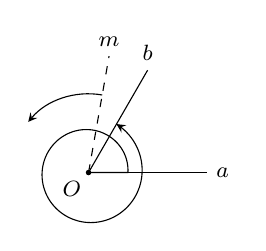
\begin{tikzpicture}[font=\footnotesize, >=stealth, declare function={r=0.5;dau=0;cuoi=60+360;}, baseline=(current bounding box.south)]
			\draw (0,0)--(1.5,0)node[right]{$a$};
			\draw[dashed] (0,0)--(80:1.5)node[above]{$m$};
			\draw[->] (80:1) arc (80:140:1);
			\draw[smooth, samples=200, ->] (0,0)--plot[domain=dau:cuoi] (\x:r+\x/2000)coordinate (B);
			\draw (0,0)--(cuoi:1.5)node[above]{$b$};
			\fill (0,0) circle (1pt)+(-135:0.3)node{$O$};
		\end{tikzpicture}
		&
		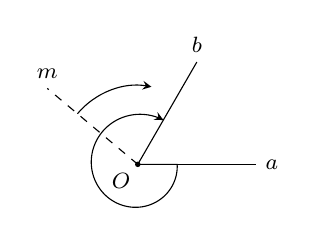
\begin{tikzpicture}[font=\footnotesize, >=stealth, declare function={r=0.5;dau=0;cuoi=60;}, baseline=(current bounding box.south)]
			\draw (0,0)--(1.5,0)node[right]{$a$};
			\draw[dashed] (0,0)--(140:1.5)node[above]{$m$};
			\draw[->] (140:1) arc (140:80:1);
			\draw[smooth, samples=200, ->] (0,0)--plot[domain=0:-360+cuoi] (\x:r-\x/2000)coordinate (B);
			\draw (0,0)--(cuoi:1.5)node[above]{$b$};
			\fill (0,0) circle (1pt)+(-135:0.3)node{$O$};
		\end{tikzpicture}
	\end{tabular}
\end{dn}
\begin{note}
	Với hai tia $Oa$ và $Ob$ cho trước, có vô số góc lượng giác tia đầu $Oa$ và tia cuối $Ob$. Ta dùng chung kí hiệu $(Oa,Ob)$ cho tất cả các góc lượng giác này.
\end{note}
\begin{nx}
	Số đo của các góc lượng giác có cùng tia đầu $Oa$ và tia cuối $Ob$ khác nhau một bội nguyên của $360^\circ$ nên có công thức tổng quát là:
	\begin{center}
		$\text{sđ}(Oa,Ob)=\alpha^\circ+k\cdot360^\circ$ ($k\in\mathbb{Z}$), thường viết là $(Oa, Ob)=\alpha^\circ+k\cdot360^\circ$.
	\end{center}
\end{nx}
\begin{dl}
	(Hệ thức Chasles) Với ba tia Oa, Ob và Oc bất kì, ta có:
	$$(Oa,Ob)+(Ob,Oc)=(Oa,Oc)+k\cdot360^\circ\,\,(k\in\mathbb{Z}).$$
\end{dl}
\subsubsection{Đơn vị radian}
\begin{dn}
	\immini
	{Trên đường tròn bán kính $R$ tùy ý, góc ở tâm chắn một cung có độ dài đúng bằng $R$ được gọi là một góc có số đo $1$ radian (viết tắt là $1$ rad).}
	{
	\begin{tikzpicture}[font=\footnotesize, >=stealth, declare function={r=1.5;}]
		\path (0,0) coordinate (O) (r,0) coordinate (A) (180/pi:r) coordinate (B)
		pic[draw, angle radius=2mm,"$\alpha$", angle eccentricity=2]{angle=A--O--B};
		\draw (0,0) circle (r) (A)--(O)node[below,midway]{$R$}--(B);
		\draw (90/pi:r)node[right]{$R$};
	\end{tikzpicture}
	}
\end{dn}
\begin{nx}
	Vì góc bẹt ($180^\circ$) chắn nửa đường tròn với độ dài là $\pi R$, nên góc bẹt có số đo theo radian là $\pi$. Khi đó ta viết
	$$180^\circ=\pi\,\text{rad}.$$
	Do đó ta có công thức chuyển đổi số đo góc từ đơn vị radian sang độ và ngược lại như sau:
	\begin{multicols}{2}
		\begin{itemize}
			\item $a^\circ=\dfrac{\pi a}{180}$ rad
			\item $\alpha\,\text{rad}=\left(\dfrac{180\alpha}{\pi}\right)^\circ$
		\end{itemize}
	\end{multicols}
\end{nx}
\begin{note}
	\begin{itemize}
		\item Khi ghi số đo của một góc theo đơn vị radian, người ta thường bỏ đi chữ rad sau số đo.
		\item Với đơn vị radian, công thức số đo tổng quát của một góc lượng giác $(Oa, Ob)$ là
		$$(Oa, Ob) = \alpha+k2\pi\,\, (k\in\mathbb{Z}),$$
		trong đó $\alpha$ là số đo theo radian của một góc lượng giác bất kì có tia đầu $Oa$ và tia cuối $Ob$.
		\item Không được viết $\alpha+k360^\circ$ hay $\alpha^\circ+k2\pi$ vì không cùng đơn vị.
	\end{itemize}
\end{note}
\begin{dl}
	Một cung tròn của một đường tròn bán kính $R$ có số đo $\alpha$ rad thì có độ dài
	\begin{center}
		$\ell=R\alpha$.
	\end{center}
	Nếu số đo góc là $a^\circ$ thì độ dài cung có độ dài là
	\begin{center}
		$\ell=\dfrac{\pi Ra}{180}$.
	\end{center}
\end{dl}
\subsubsection{Đường tròn lượng giác}
\begin{dn}
	\immini
	{Trong mặt phẳng tọa độ $Oxy$, cho đường tròn tâm $O$ bán kính bằng $1$. Trên đường tròn này, chọn điểm $A(1; 0)$ làm gốc, chiều dương là chiều ngược chiều kim đồng hồ và chiều âm là chiều cùng chiều kim đồng hồ. Đường tròn cùng với gốc và chiều như trên được gọi là \textbf{đường tròn lượng giác}.}
	{
	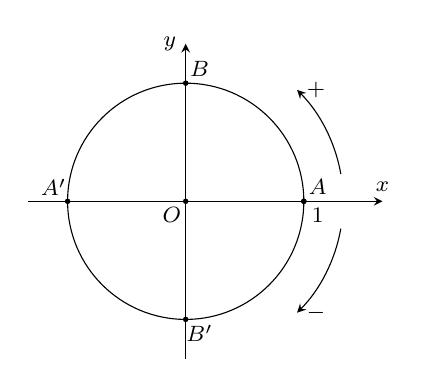
\begin{tikzpicture}[font=\footnotesize, >=stealth, declare function={r=1.5;}]
		\path (0,0) coordinate (O) (0:r) coordinate (A) (180:r) coordinate (A') (90:r) coordinate (B) (-90:r) coordinate (B');
		\draw[->] (-r-0.5,0)--(r+1,0)node[above]{$x$};
		\draw[->] (0,-r-0.5)--(0,r+0.5)node[left]{$y$};
		\draw[->] (10:r+0.5) arc (10:45:r+0.5)node[right]{$+$};
		\draw[->] (-10:r+0.5) arc (-10:-45:r+0.5)node[right]{$-$};
		\fill (r,0) circle (1pt)+(-45:0.25)node{$1$};
		\draw (O) circle (r);
		\foreach \x/\g in {O/-135, A/45, B/45, A'/135, B'/-45}{
		\fill (\x) circle (1pt)+(\g:0.25)node{$\x$};
		}
	\end{tikzpicture}
	}
\end{dn}
\newpage
\begin{dn}
	Cho số đo góc $\alpha$ bất kì. Trên đường tròn lượng giác, ta xác định được duy nhất một điểm $M$ sao cho số đo góc lượng giác $(OA, OM)$ bằng $\alpha$. Khi đó $M$ được gọi là \textbf{điểm biểu diễn} của góc có số đo $\alpha$ trên đường tròn lượng giác.
\end{dn}
\begin{note}
	Hệ trục tọa độ $Oxy$ chia mặt phẳng tọa độ thành bốn \lq\lq góc phần tư\rq\rq\, kí hiệu lần lượt là I, II, III và IV.\\
	\begin{tabular}{C{0.5\linewidth}C{0.5\linewidth}}
		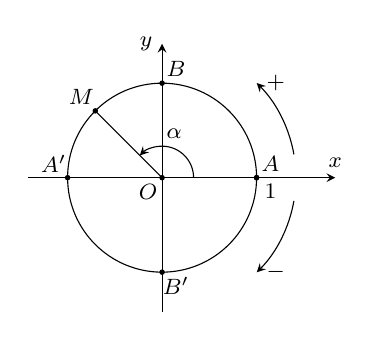
\begin{tikzpicture}[font=\footnotesize, >=stealth, declare function={r=1.2;}]
			\path (0,0) coordinate (O) (0:r) coordinate (A) (180:r) coordinate (A') (90:r) coordinate (B) (-90:r) coordinate (B') (135:r) coordinate (M);
			\draw[->] (-r-0.5,0)--(r+1,0)node[above]{$x$};
			\draw[->] (0,-r-0.5)--(0,r+0.5)node[left]{$y$};
			\draw[->] (0:r/3) arc (0:135:r/3)node[above, midway]{$\alpha$};
			\draw[->] (10:r+0.5) arc (10:45:r+0.5)node[right]{$+$};
			\draw[->] (-10:r+0.5) arc (-10:-45:r+0.5)node[right]{$-$};
			\fill (r,0) circle (1pt)+(-45:0.25)node{$1$};
			\draw (O) circle (r) (O)--(M);
			\foreach \x/\g in {O/-135, A/45, B/45, A'/135, B'/-45, M/135}{
			\fill (\x) circle (1pt)+(\g:0.25)node{$\x$};
			}
		\end{tikzpicture}
		&
		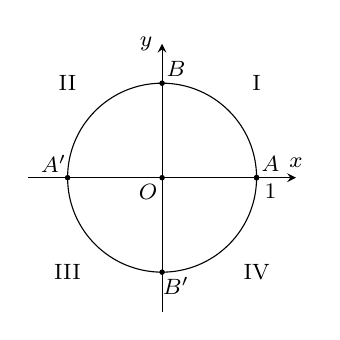
\begin{tikzpicture}[font=\footnotesize, >=stealth, declare function={r=1.2;}]
			\path (0,0) coordinate (O) (0:r) coordinate (A) (180:r) coordinate (A') (90:r) coordinate (B) (-90:r) coordinate (B');
			\draw[->] (-r-0.5,0)--(r+0.5,0)node[above]{$x$};
			\draw[->] (0,-r-0.5)--(0,r+0.5)node[left]{$y$};
			\fill (r,0) circle (1pt)+(-45:0.25)node{$1$};
			\draw (O) circle (r);
			\foreach \x/\g in {O/-135, A/45, B/45, A'/135, B'/-45}{
			\fill (\x) circle (1pt)+(\g:0.25)node{$\x$};
			}
			\draw (45:r+0.5) node{I} (135:r+0.5) node{II} (-135:r+0.5) node{III} (-45:r+0.5) node{IV};
		\end{tikzpicture}
	\end{tabular}
\end{note}
\subsubsection{Giá trị lượng giác của góc lượng giác}
\begin{dn}
	Trên đường tròn lượng giác, gọi $M(x_M;y_M)$ là điểm biểu diễn góc lượng giác có số đo $\alpha$. Khi đó
	\immini
	{
	\begin{enumerate}[\iconMT]
		\item Tung độ $y_M$ của điểm $M$ gọi là \textbf{\textit{sin}} của $\alpha$, kí hiệu $\sin\alpha$.
		\item Hoành độ $x_M$ của điểm $M$ gọi là \textbf{\textit{côsin}} của $\alpha$, kí hiệu $\cos\alpha$.
		\item Nếu $x_M\ne0$ thì tỉ số $\dfrac{y_M}{x_M}=\dfrac{\sin\alpha}{\cos\alpha}$ gọi là \textbf{\textit{tang}} của góc $\alpha$, kí hiệu $\tan\alpha$.
		\item Nếu $y_M\ne0$ thì tỉ số $\dfrac{x_M}{y_M}=\dfrac{\cos\alpha}{\sin\alpha}$ gọi là \textbf{\textit{côtang}} của góc $\alpha$, kí hiệu $\cot\alpha$.
	\end{enumerate}
	}
	{
	\begin{tikzpicture}[font=\footnotesize, >=stealth, declare function={r=1.2;}]
		\path (0,0) coordinate (O) (0:r) coordinate (A) (180:r) coordinate (A') (90:r) coordinate (B) (-90:r) coordinate (B') (45:r) coordinate (M);
		\draw[->] (-r-0.5,0)--(r+0.5,0)node[above]{$x$};
		\draw[->] (0,-r-0.5)--(0,r+0.5)node[left]{$y$};
		\draw[->] (0:r/3) arc (0:45:r/3)node[right, midway]{$\alpha$};
		\fill (r,0) circle (1pt)+(-45:0.25)node{$1$};
		\draw (O) circle (r) (O)--(M);
		\foreach \x/\g in {O/-135, A/45, B/45, A'/135, B'/-45, M/45}{
		\fill (\x) circle (1pt)+(\g:0.25)node{$\x$};
		}
		\path
		($(O)!(M)!(A)$) coordinate (Mx) ($(O)!(M)!(B)$) coordinate (My);
		\fill (Mx) circle(1pt)node[below]{$x_M$} (My)circle(1pt)node[left]{$y_M$};
		\draw[dashed] (Mx)|-(My);
	\end{tikzpicture}
	}
	Các giá trị $\sin\alpha$, $\cos\alpha$, $\tan\alpha$, $\cot\alpha$ được gọi là \textit{các giá trị lượng giác của góc lượng giác} $\alpha$.
\end{dn}
\begin{note}
	\begin{enumerate}
		\item Ta gọi trục hoành là \textbf{\textit{trục côsin}}, còn trục tung là \textbf{\textit{trục sin}}.
		\item Trục $At$ có gốc ở điểm $A(1; 0)$ và song song với trục sin gọi là \textbf{\textit{trục tang}}.\\
		Nếu đường thẳng $OM$ cắt trục tang thì tung độ của giao điểm đó chính là $\tan\alpha$.
		\item Trục $Bs$ có gốc ở điểm $B(0; 1)$ và song song với trục côsin gọi là \textbf{\textit{trục côtang}}. Nếu đường thẳng $OM$ cắt trục côtang thì hoành độ của giao điểm đó chính là $\cot\alpha$.\\
		\begin{tabular}{C{0.5\linewidth}C{0.5\linewidth}}
			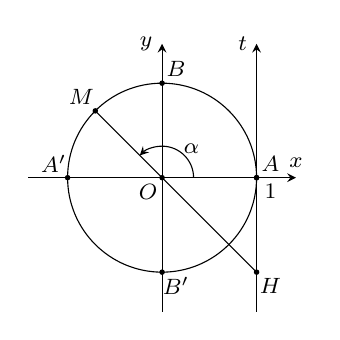
\begin{tikzpicture}[font=\footnotesize, >=stealth, declare function={r=1.2;}]
				\path (0,0) coordinate (O) (0:r) coordinate (A) (180:r) coordinate (A') (90:r) coordinate (B) (-90:r) coordinate (B') (135:r) coordinate (M)
				(r,r) coordinate (a);
				\draw[->] (-r-0.5,0)--(r+0.5,0)node[above]{$x$};
				\draw[->] (0,-r-0.5)--(0,r+0.5)node[left]{$y$};
				\draw[->] (0:r/3) arc (0:135:r/3)node[right, midway]{$\alpha$};
				\fill (r,0) circle (1pt)+(-45:0.25)node{$1$};
				\draw (O) circle (r) (O)--(M);
				\path (intersection of O--M and A--a) coordinate (H);
				\draw[->] (r,-r-0.5)--(r,r+0.5)node[left]{$t$};
				\draw (O)--(H);
				\foreach \x/\g in {O/-135, A/45, B/45, A'/135, B'/-45, M/135, H/-45}{
				\fill (\x) circle (1pt)+(\g:0.25)node{$\x$};
				}
			\end{tikzpicture}
			&
			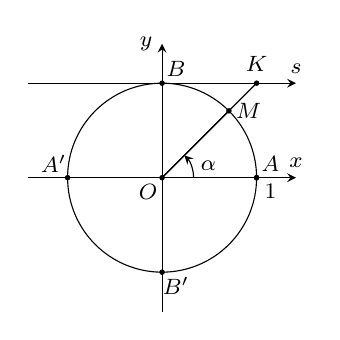
\begin{tikzpicture}[font=\footnotesize, >=stealth, declare function={r=1.2;}]
				\path (0,0) coordinate (O) (0:r) coordinate (A) (180:r) coordinate (A') (90:r) coordinate (B) (-90:r) coordinate (B') (45:r) coordinate (M)
				(r,r) coordinate (a);
				\draw[->] (-r-0.5,0)--(r+0.5,0)node[above]{$x$};
				\draw[->] (0,-r-0.5)--(0,r+0.5)node[left]{$y$};
				\draw[->] (0:r/3) arc (0:45:r/3)node[right, midway]{$\alpha$};
				\fill (r,0) circle (1pt)+(-45:0.25)node{$1$};
				\draw (O) circle (r) (O)--(M);
				\path (intersection of O--M and B--a) coordinate (K);
				\draw[->] (-r-0.5,r)--(r+0.5,r)node[above]{$s$};
				\draw (O)--(K);
				\foreach \x/\g in {O/-135, A/45, B/45, A'/135, B'/-45, M/0, K/90}{
				\fill (\x) circle (1pt)+(\g:0.25)node{$\x$};
				}
			\end{tikzpicture}
		\end{tabular}
		\item $\sin\alpha$ và $\cos\alpha$ xác định với mọi $\alpha\in\mathbb{R}$;\\
		$\tan\alpha$ chỉ xác định với các góc $\alpha\ne\dfrac{\pi}{2}+k\pi$ ($k\in\mathbb{Z}$);\\
		$\cot\alpha$ chỉ xác định với các góc $\alpha\ne k\pi$ ($k\in\mathbb{Z}$).
		\item Ta đã biết bảng giá trị lượng giác của một số góc $\alpha$ đặc biệt với $0\leq\alpha\leq\dfrac{\pi}{2}$ (hay $0^\circ\leq\alpha\leq90^\circ$) như sau
		\begin{center}
			\begin{tabular}{|c|c|c|c|c|c|}
				\hline
				\multirow{2}{*}{$\alpha$}
				& $0$ & $\dfrac{\pi}{6}$ & $\dfrac{\pi}{4}$ & $\dfrac{\pi}{3}$ & $\dfrac{\pi}{2}$ \\
				& ($0^\circ$) & ($30^\circ$) & ($45^\circ$) & ($60^\circ$) & ($90^\circ$) \\
				\hline
				$\sin\alpha$ & $0$ & $\dfrac{1}{2}$ & $\dfrac{\sqrt2}{2}$ & $\dfrac{\sqrt3}{2}$ & $1$ \\
				\hline
				$\cos\alpha$ & $1$ & $\dfrac{\sqrt3}{2}$ & $\dfrac{\sqrt2}{2}$ & $\dfrac{1}{2}$ & $0$ \\
				\hline
				$\tan\alpha$ & $0$ & $\dfrac{1}{\sqrt3}$ & $1$ & $\sqrt3$ & \raisebox{-0.5ex}{\tikz \draw (0,-0.25) -- (0,0.25) (0.1,-0.25)--(0.1,0.25);} \\
				\hline
				$\cot\alpha$ & \raisebox{-0.5ex}{\tikz \draw (0,-0.25) -- (0,0.25) (0.1,-0.25)--(0.1,0.25);} & $\sqrt3$ & $1$ & $\dfrac{1}{\sqrt3}$ & $0$ \\
				\hline
			\end{tabular}
		\end{center}
		\item Ta có thể sử dụng đường tròn lượng giác để xác định giá trị lượng giác của góc $\alpha$.\\
		\begin{tabular}{C{0.5\linewidth}C{0.5\linewidth}}
			\begin{tikzpicture}[font=\footnotesize, >=stealth, declare function={r=2;}]
				\path (0,0) coordinate (O) (0:r) coordinate (A) (180:r) coordinate (A') (90:r) coordinate (B) (-90:r) coordinate (B');
				\draw[->] (-r-0.5,0)--(r+1,0)node[above]{$x$};
				\draw[->] (0,-r-0.5)--(0,r+1)node[left]{$y$};
				\draw (O) circle (r);
				\draw[dashed] (-150:r) rectangle (30:r) (-135:r) rectangle (45:r) (-120:r) rectangle (60:r);
				\foreach \x/\g/\n in {0/45/0 ,30/30/{\dfrac{\pi}{6}}, 45/45/{\dfrac{\pi}{4}}, 60/60/{\dfrac{\pi}{3}}, 90/45/{\dfrac{\pi}{2}}, 120/120/{\dfrac{2\pi}{3}}, 135/135/{\dfrac{3\pi}{4}}, 150/150/{\dfrac{5\pi}{6}}, 180/135/{\pi}, 270/-135/{\dfrac{3\pi}{2}}, 360/-30/{2\pi} }{
				\fill (\x:r) circle (1pt)+(\g:0.4)node{$\n$};
				}
				\foreach \x/\g/\n in {-30/-30/{-\dfrac{\pi}{6}}, -45/-45/{-\dfrac{\pi}{4}}, -60/-60/{-\dfrac{\pi}{3}}, -90/-45/{-\dfrac{\pi}{2}}, -120/-120/{-\dfrac{2\pi}{3}}, -135/-135/{-\dfrac{3\pi}{4}}, -150/-150/{-\dfrac{5\pi}{6}}, -180/-150/{-\pi} }{
				\fill (\x:r) circle (1pt)+(\g:0.5)node{$\n$};
				}
				\fill (O) circle (1pt)node[below left]{$O$};
			\end{tikzpicture}
			&
			\begin{tikzpicture}[font=\footnotesize, >=stealth, declare function={r=2;}]
				\path (0,0) coordinate (O) (0:r) coordinate (A) (180:r) coordinate (A') (90:r) coordinate (B) (-90:r) coordinate (B');
				\draw[->] (-r-0.5,0)--(r+1,0)node[above]{$x$};
				\draw[->] (0,-r-0.5)--(0,r+1)node[left]{$y$};
				\draw (O) circle (r);
				\draw[dashed] (-150:r) rectangle (30:r) (-135:r) rectangle (45:r) (-120:r) rectangle (60:r);
				\foreach \x/\g/\n in {0/45/0 ,30/30/{\tfrac{\pi}{6}}, 45/45/{\tfrac{\pi}{4}}, 60/60/{\tfrac{\pi}{3}}, 90/45/{\tfrac{\pi}{2}}, 120/120/{\tfrac{2\pi}{3}}, 135/135/{\tfrac{3\pi}{4}}, 150/150/{\tfrac{5\pi}{6}}, 180/135/{\pi}, 270/-135/{\tfrac{3\pi}{2}}, 360/-30/{2\pi} }{
				\fill (\x:r) circle (1pt)+(\g:0.3)node{$\x$};
				}
				\foreach \x/\g/\n in {-30/-30/{-\tfrac{\pi}{6}}, -45/-45/{-\tfrac{\pi}{4}}, -60/-60/{-\tfrac{\pi}{3}}, -90/-45/{-\tfrac{\pi}{2}}, -120/-120/{-\tfrac{2\pi}{3}}, -135/-135/{-\tfrac{3\pi}{4}}, -150/-150/{-\tfrac{5\pi}{6}}, -180/-150/{-\pi} }{
				\fill (\x:r) circle (1pt)+(\g:0.4)node{$\x$};
				}
				\fill (O) circle (1pt)node[below left]{$O$};
			\end{tikzpicture}
		\end{tabular}
	\end{enumerate}
\end{note}
\subsubsection{Hệ thức cơ bản giữa các giá trị lượng giác của một góc lượng giác}
\begin{dl}
	Cho góc lượng giác $\alpha$.
	\begin{enumerate}[\iconMT]
		\item Với mọi $\alpha$ ta có $\sin^2\alpha+\cos^2\alpha=1$.
		\item Với $\alpha\ne\dfrac{k\pi}{2}$ ($k\in\mathbb{Z}$) ta có $\tan\alpha\cdot\cot\alpha=1$.
		\item Với $\alpha\ne\dfrac{\pi}{2}+k\pi$ ($k\in\mathbb{Z}$) ta có $1+\tan^2\alpha=\dfrac{1}{\cos^2\alpha}$.
		\item Với $\alpha\ne k\pi$ ($k\in\mathbb{Z}$) ta có $1+\cot^2\alpha=\dfrac{1}{\sin^2\alpha}$.
	\end{enumerate}
\end{dl}
\subsubsection{Giá trị lượng giác của các góc lượng giác có liên quan đặc biệt}
\begin{enumerate}[\iconMT]
	\item\indam{Hai góc đối nhau:}
	\begin{boxdn}
		\immini
		{
		\begin{itemize}
			\item $\cos(-\alpha)=\cos\alpha$
			\item $\sin(-\alpha)=-\sin(\alpha)$
			\item $\tan(-\alpha)=-\tan(\alpha)$
			\item $\cot(-\alpha)=-\cot(\alpha)$
		\end{itemize}
		}
		{
		\begin{tikzpicture}[font=\footnotesize, >=stealth, declare function={r=1.5;cuoi=45;}]
			\path (0,0) coordinate (O) (0:r) coordinate (A) (180:r) coordinate (A') (90:r) coordinate (B) (-90:r) coordinate (B') (cuoi:r) coordinate (M) (-cuoi:r) coordinate (N);
			\draw[->] (-r-0.5,0)--(r+0.5,0)node[above]{$x$};
			\draw[->] (0,-r-0.5)--(0,r+0.5)node[left]{$y$};
			\draw[->] (0:r/3) arc (0:cuoi:r/3)node[right, midway]{$\alpha$};
			\draw[->] (0:r/4) arc (0:-cuoi:r/4)node[right, midway]{$-\alpha$};
			\fill (r,0) circle (1pt)+(-45:0.25)node{$1$};
			\draw (O) circle (r) (N)--(O)--(M);
			\foreach \x/\g in {O/-135, A/45, B/45, A'/135, B'/-45, M/cuoi, N/-cuoi}{
			\fill (\x) circle (1pt)+(\g:0.25)node{$\x$};
			}
			\path
			($(O)!(M)!(A)$) coordinate (Mx);
			\fill (Mx)circle(1pt);
			\draw[dashed] (M)--(N);
		\end{tikzpicture}
		}
	\end{boxdn}
	\item\indam{Hai góc bù nhau:}
	\begin{boxdn}
		\immini
		{
		\begin{itemize}
			\item $\sin(\pi-\alpha)=\sin(\alpha)$
			\item $\cos(\pi-\alpha)=-\cos(\alpha)$
			\item $\tan(\pi-\alpha)=-\tan(\alpha)$
			\item $\cot(\pi-\alpha)=-\cot(\alpha)$
		\end{itemize}
		}
		{
		\begin{tikzpicture}[font=\footnotesize, >=stealth, declare function={r=1.5;cuoi=45;}]
			\path (0,0) coordinate (O) (0:r) coordinate (A) (180:r) coordinate (A') (90:r) coordinate (B) (-90:r) coordinate (B') (cuoi:r) coordinate (M) (180-cuoi:r) coordinate (N);
			\draw[->] (-r-0.5,0)--(r+0.5,0)node[above]{$x$};
			\draw[->] (0,-r-0.5)--(0,r+0.5)node[left]{$y$};
			\draw[->] (0:r/3) arc (0:cuoi:r/3)node[right, midway]{$\alpha$};
			\draw[->] (0:r/4) arc (0:180-cuoi:r/4)node[above, midway]{$\pi-\alpha$};
			\fill (r,0) circle (1pt)+(-45:0.25)node{$1$};
			\draw (O) circle (r) (N)--(O)--(M);
			\foreach \x/\g in {O/-45, A/45, B/45, A'/135, B'/-45, M/cuoi, N/180-cuoi}{
			\fill (\x) circle (1pt)+(\g:0.25)node{$\x$};
			}
			\path
			($(O)!(M)!(B)$) coordinate (Mx) ($(O)!(N)!(B)$) coordinate (Nx);
			\fill (Mx)circle(1pt);
			\draw[dashed] (M)--(N);
		\end{tikzpicture}
		}
	\end{boxdn}
	\item\indam{Hai góc phụ nhau:}
	\begin{boxdn}
		\immini
		{
		\begin{itemize}
			\item $\sin\left(\dfrac{\pi}{2}-\alpha\right)=\cos(\alpha)$
			\item $\cos\left(\dfrac{\pi}{2}-\alpha\right)=\sin(\alpha)$
			\item $\tan\left(\dfrac{\pi}{2}-\alpha\right)=\cot(\alpha)$
			\item $\cot\left(\dfrac{\pi}{2}-\alpha\right)=\tan(\alpha)$
		\end{itemize}
		}
		{
		\begin{tikzpicture}[font=\footnotesize, >=stealth, declare function={r=1.5;cuoi=30;}]
			\path (0,0) coordinate (O) (0:r) coordinate (A) (180:r) coordinate (A') (90:r) coordinate (B) (-90:r) coordinate (B') (cuoi:r) coordinate (M) (90-cuoi:r) coordinate (N);
			\draw[->] (-r-0.5,0)--(r+0.5,0)node[above]{$x$};
			\draw[->] (0,-r-0.5)--(0,r+0.5)node[left]{$y$};
			\draw[->] (0:r/3) arc (0:cuoi:r/3);
			\draw[->] (0:r/4) arc (0:90-cuoi:r/4);
			\fill (r,0) circle (1pt)+(-45:0.25)node{$1$};
			\draw (O) circle (r) (N)--(O)--(M);
			\foreach \x/\g in {O/-45, A/45, B/45, A'/135, B'/-45, M/cuoi, N/90-cuoi}{
			\fill (\x) circle (1pt)+(\g:0.25)node{$\x$};
			}
			\path
			($(O)!(M)!(A)$) coordinate (Mx) ($(O)!(M)!(B)$) coordinate (My)
			($(O)!(N)!(A)$) coordinate (Nx) ($(O)!(N)!(B)$) coordinate (Ny);;
			\fill (Mx)circle(1pt) (Nx)circle(1pt) (My)circle(1pt) (Ny)circle(1pt);
			\draw[dashed] (Mx)|-(My) (Nx)|-(Ny);
		\end{tikzpicture}
		}
	\end{boxdn}
	\item\indam{Hai góc hơn, kém $\pi$:}
	\begin{boxdn}
		\immini
		{
		\begin{itemize}
			\item $\tan(\alpha+\pi)=\tan(\alpha)$
			\item $\cot(\alpha+\pi)=\cot(\alpha)$
			\item $\sin(\alpha+\pi)=-\sin(\alpha)$
			\item $\cos(\alpha+\pi)=-\cos(\alpha)$
		\end{itemize}
		}
		{
		\begin{tikzpicture}[font=\footnotesize, >=stealth, declare function={r=1.5;cuoi=45;}]
			\path (0,0) coordinate (O) (0:r) coordinate (A) (180:r) coordinate (A') (90:r) coordinate (B) (-90:r) coordinate (B') (cuoi:r) coordinate (M) (cuoi+180:r) coordinate (N);
			\draw[->] (-r-0.5,0)--(r+0.5,0)node[above]{$x$};
			\draw[->] (0,-r-0.5)--(0,r+0.5)node[left]{$y$};
			\draw[->] (0:r/3) arc (0:cuoi:r/3)node[right, midway]{$\alpha$};
			\draw[->] (0:r/4) arc (0:cuoi+180:r/4)node[above, midway]{$\alpha+\pi$};
			\fill (r,0) circle (1pt)+(-45:0.25)node{$1$};
			\draw (O) circle (r) (N)--(O)--(M);
			\foreach \x/\g in {O/-45, A/45, B/45, A'/135, B'/-45, M/cuoi, N/cuoi+180}{
			\fill (\x) circle (1pt)+(\g:0.25)node{$\x$};
			}
			\path
			($(O)!(M)!(A)$) coordinate (Mx) ($(O)!(N)!(A)$) coordinate (Nx);
			\fill (Mx)circle(1pt) (Nx)circle(1pt);
			\draw[dashed] (M)--(Mx)node[below]{$x_0$} (N)--(Nx)node[above]{$-x_0$};
		\end{tikzpicture}
		}
	\end{boxdn}
\end{enumerate}
%-------------------------------------------------------------------------------------------------------------
\subsection{PHÂN LOẠI VÀ PHƯƠNG PHÁP GIẢI TOÁN}
\begin{dang}{Góc lượng giác}
\end{dang}
%%% Ví dụ 1
\begin{vd}
	%\textit{(Trích )}
	Hãy hoàn thành bảng chuyển đổi số đo độ và số so radian của một góc sau
	\begin{center}
		\begin{tabular}{|c|C{10mm}|C{10mm}|C{10mm}|C{10mm}|C{10mm}|C{10mm}|}
			\hline
			Độ 	& $18^\circ$ 	& 	& $72^\circ$ 	& 	& $130^\circ$ 	& \\
			\hline
			Radian 	& 	& $\dfrac{2\pi}{9}$ 	& 	& $\dfrac{5\pi}{9}$ 	& 	& $\dfrac{5\pi}{6}$  \\
			\hline
		\end{tabular}
	\end{center}
\loigiai{
	\begin{center}
		\begin{tabular}{|c|C{10mm}|C{10mm}|C{10mm}|C{10mm}|C{10mm}|C{10mm}|}
			\hline
			Độ 	& $18^\circ$ 	& $40^\circ$ 	& $72^\circ$ 	& $100^\circ$ 	& $130^\circ$ 	& $150^\circ$ \\
			\hline
			Radian 	& $\dfrac{\pi}{10}$ 	& $\dfrac{2\pi}{9}$ 	& $\dfrac{2\pi}{5}$ 	& $\dfrac{5\pi}{9}$ 	& $\dfrac{13\pi}{18}$ 	& $\dfrac{5\pi}{6}$  \\
			\hline
		\end{tabular}
	\end{center}
	}
\end{vd}
%%% Ví dụ 2
\begin{vd}
	%\textit{(Trích )}
	Hãy biểu diễn các góc lượng sau trên đường tròn lượng giác
	\begin{multicols}{4}
		\begin{enumerate}
			\item $\dfrac{2\pi}{3}$;
			\item $\dfrac{13\pi}{3}$;
			\item $-\dfrac{25\pi}{12}$;
			\item $-\dfrac{27\pi}{4}$.
		\end{enumerate}
	\end{multicols}
\loigiai{
	\immini
	{
	\begin{enumerate}
		\item Gọi $M$ là điểm biểu diễn của góc lượng có số đo $\dfrac{2\pi}{3}$.
		\item Ta có $\dfrac{13\pi}{3}=\dfrac{\pi}{3}+2\cdot2\pi$.\\
		Gọi $N$ là điểm biểu diễn của góc có số đó $\dfrac{\pi}{3}$.\\
		Khi đó góc có số đo $\dfrac{13\pi}{3}$ cũng được biểu diễn bởi điểm $N$.
		\item Ta có $-\dfrac{25\pi}{12}=-\dfrac{\pi}{12}-2\pi$.\\
		Gọi $P$ là điểm biểu diễn của góc lượng có số đo $-\dfrac{\pi}{12}$.\\
		Khi đó góc có số đo $-\dfrac{25\pi}{12}$ cũng được biểu diễn bởi điểm $P$.
		\item Ta có $-\dfrac{27\pi}{4}=-\dfrac{3\pi}{4}-3\cdot2\pi$.\\
		Gọi $Q$ là điểm biểu diễn của góc lượng có số đo $-\dfrac{3\pi}{4}$.\\
		Khi đó góc có số đo $-\dfrac{27\pi}{4}$ cũng được biểu diễn bởi điểm $Q$.
	\end{enumerate}
	}
	{
	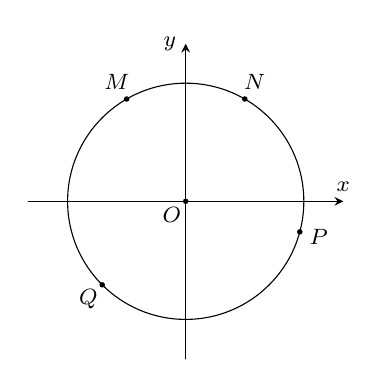
\begin{tikzpicture}[font=\footnotesize, line join=round, line cap=round, >=stealth, scale=1, declare function={r=1.5;}]
		\path (0,0) coordinate (O) (120:r) coordinate (M) (60:r) coordinate (N) (-15:r) coordinate (P) (-135:r) coordinate (Q);
		\draw[->] (-r-0.5,0)--(r+0.5,0)node[above]{$x$};
		\draw[->] (0,-r-0.5)--(0,r+0.5)node[left]{$y$};
		\draw (O) circle (r);
		\foreach \x/\g in {O/-135, M/120, N/60, P/-15, Q/-135}{\fill (\x) circle (1pt)+(\g:0.25)node{$\x$};}
	\end{tikzpicture}
	}
	}
\end{vd}
%%% Ví dụ 3
\begin{vd}[\textit{Trích SGK Chân trời sáng tạo}]
	Trên đường tròn lượng giác, hãy biểu diễn các góc lượng giác có số đo có dạng là
	\begin{multicols}{2}
		\begin{enumerate}
			\item $\alpha\dfrac{\pi}{2}+k\pi$ ($k\in\mathbb{Z}$);
			\item $\beta=k\dfrac{\pi}{4}$ ($k\in\mathbb{Z}$).
		\end{enumerate}
	\end{multicols}
\loigiai{
	\begin{enumerate}
		\item $\alpha=\dfrac{\pi}{2}+k\pi$ ($k\in\mathbb{Z}$).
		\immini
		{
		\begin{itemize}
			\item Với $k=0$ ta được góc có số đo là $\alpha=\dfrac{\pi}{2}$ biểu diễn bởi điểm $M$;
			\item Với $k=1$ ta được góc có số đo là $\alpha=\dfrac{3\pi}{2}$ biểu diễn bởi điểm $N$;
			\item Với $k=2$ ta được góc có số đo là $\alpha=\dfrac{\pi}{2}+2\pi$ có cùng điểm biểu diễn $M$;
			\item Với $k=3$ ta được góc có số đo là $\alpha=\dfrac{3\pi}{2}+2\pi$ có cùng điểm biểu diễn $N$.
		\end{itemize}
		Suy ra với $k$ chẵn, góc $\alpha$ được biểu diễn bởi điểm $M$, với $k$ lẻ góc $\alpha$ được biểu diễn bởi điểm $N$.}
		{
		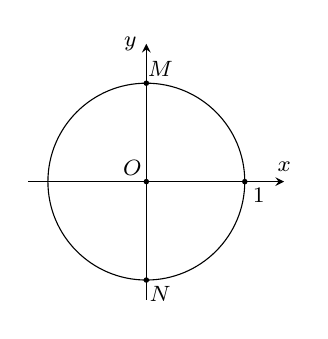
\begin{tikzpicture}[font=\footnotesize, >=stealth, declare function={r=1.25;}]
			\path (0,0) coordinate (O) (90:r) coordinate (M) (-90:r) coordinate (N);
			\draw[->] (-r-0.25,0)--(r+0.5,0)node[above]{$x$};
			\draw[->] (0,-r-0.25)--(0,r+0.5)node[left]{$y$};
			\fill (r,0) circle (1pt)+(-45:0.25)node{$1$};
			\draw (O) circle (r);
			\foreach \x/\g in {O/135, M/45, N/-45}{
			\fill (\x) circle (1pt)+(\g:0.25)node{$\x$};
			}
		\end{tikzpicture}
		}
		\item $\beta=k\dfrac{\pi}{4}$ ($k\in\mathbb{Z}$). Ta lập bảng
		\begin{center}
			\begin{tabular}{|c|c|c|c|c|c|c|c|c|c|}
				\hline
				$k$ 	& $0$ 	& $1$ 	& $2$ 	& $3$ 	& $4$ 	& $5$ 	& $6$ 	& $7$ 	& $8$ \\
				\hline
				$\beta$ 	& $0$ 	& $\dfrac{\pi}{4}$ 	& $\dfrac{\pi}{2}$ 	& $\dfrac{3\pi}{4}$ 	& $\pi$ 	& $\dfrac{5\pi}{4}$ 	& $\dfrac{3\pi}{2}$ 	& $\dfrac{7\pi}{4}$ 	& $2\pi$ \\
				\hline
				Điểm biểu diễn 	& $A$ 	& $M$ 	& $B$ 	& $N$ 	& $A'$ 	& $P$ 	& $B'$ 	& $Q$ 	& $A$ \\
				\hline
			\end{tabular}
		\end{center}
		Ta nhận thấy khi $k=8$ điểm biểu diễn của góc $\beta$ đã trùng lại với điểm $A$ khi $k=0$.\\
		Do đó góc lượng giác $\beta$ được biểu diễn bởi $8$ điểm $A$, $M$, $B$, $N$, $A'$, $P$, $B'$, $Q$ như hình
		\begin{center}
			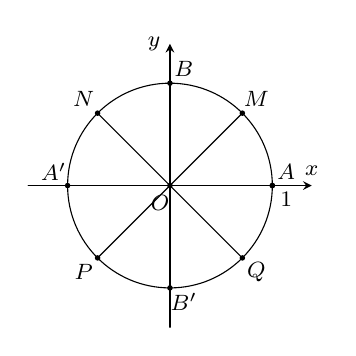
\begin{tikzpicture}[font=\footnotesize, line join=round, line cap=round, >=stealth, scale=1]
				\def\r{1.3}
				\path (0,0) coordinate (O) (0:\r) coordinate (A) (180:\r) coordinate (A') (90:\r) coordinate (B) (-90:\r) coordinate (B');
				\draw[->] (-\r-0.5,0)--(\r+0.5,0)node[above]{$x$};
				\draw[->] (0,-\r-0.5)--(0,\r+0.5)node[left]{$y$};
				\fill (\r,0) circle (1pt)+(-45:0.25)node{$1$};
				\draw (O) circle (\r);
				\foreach \x/\g in {O/-120, A/45, B/45, A'/135, B'/-45}{\fill (\x) circle (1pt)+(\g:0.25)node{$\x$};}
				\foreach \x [count=\i from 0] in {M,N,P,Q}{\draw (O)--(45+90*\i:\r);
				\fill (45+90*\i:\r) circle (1pt)+(45+90*\i:0.25)node{$\x$};}
			\end{tikzpicture}
		\end{center}
	\end{enumerate}
	}
\end{vd}
\begin{dang}{Giá trị lượng giác của một góc}
\end{dang}
%%% Ví dụ 4
\begin{vd}
	%\textit{(Trích )}
	Trên đường tròn lượng giác cho góc lượng giác $\alpha$ được biểu diễn bởi điểm $M$ được biểu diễn như hình vẽ sau
	\begin{center}
		\begin{tikzpicture}[font=\footnotesize, >=stealth, declare function={r=2;}]
			\path (0,0) coordinate (O) (0:r) coordinate (A) (180:r) coordinate (A') (90:r) coordinate (B) (-90:r) coordinate (B') (-120:r) coordinate (M);
			\draw[->] (-r-0.5,0)--(r+0.5,0)node[above]{$x$};
			\draw[->] (0,-r-0.5)--(0,r+0.5)node[left]{$y$};
			\draw[->] (0:r/4) arc (0:-120:r/4)node[right, midway]{$\alpha$};
			\fill (r,0) circle (1pt)+(-45:0.25)node{$1$};
			\draw (O) circle (r) (O)--(M);
			\foreach \x/\g in {O/135, A/45, M/-120}{
			\fill (\x) circle (1pt)+(\g:0.25)node{$\x$};
			}
			\path
			($(O)!(M)!(A)$) coordinate (Mx) ($(O)!(M)!(B)$) coordinate (My);
			\fill (Mx) circle(1pt)node[above]{$-\dfrac{1}{2}$} (My)circle(1pt)node[above right=-1mm]{$-\dfrac{\sqrt3}{2}$};
			\draw[dashed] (Mx)|-(My);
		\end{tikzpicture}
	\end{center}
	Xác định các giá trị lượng giác của góc $\alpha$.
\loigiai{
	Điểm $M$ có tọa độ $(x_M;y_M)=\left(-\dfrac{1}{2};-\dfrac{\sqrt3}{2}\right)$. Khi đó ta có
	\begin{multicols}{4}
		\begin{itemize}
			\item $\sin\alpha=y_M=-\dfrac{\sqrt3}{2}$;
			\item $\cos\alpha=x_M=-\dfrac{1}{2}$;
			\item $\tan\alpha=\dfrac{y_M}{x_M}=\sqrt3$;
			\item $\cot\alpha=\dfrac{x_M}{y_M}=\dfrac{1}{\sqrt3}$.
		\end{itemize}
	\end{multicols}
	}
\end{vd}
%%% Ví dụ 5
\begin{vd}
	%\textit{(Trích )}
	Tính giá trị của góc lượng giác có số đo $\dfrac{\pi}{6}+k2\pi$ ($k\in\mathbb{Z}$).
\loigiai{
	Ta có
	\begin{multicols}{2}
		\begin{itemize}
			\item $\sin\left(\dfrac{\pi}{6}+k2\pi\right)=\sin\dfrac{\pi}{6}=\dfrac{1}{2}$;
			\item $\cos\left(\dfrac{\pi}{6}+k2\pi\right)=\cos\dfrac{\pi}{6}=\dfrac{\sqrt3}{2}$;
			\item $\tan\left(\dfrac{\pi}{6}+k2\pi\right)=\tan\dfrac{\pi}{6}=\dfrac{1}{\sqrt3}$;
			\item $\cot\left(\dfrac{\pi}{6}+k2\pi\right)=\cot\dfrac{\pi}{6}=\sqrt3$.
		\end{itemize}
	\end{multicols}
	}
\end{vd}
\begin{dang}{Áp dụng tính chất của giá trị lượng giác}
\end{dang}
%%% Ví dụ 6
\begin{vd}
	%\textit{(Trích )}
	Tính giá trị lượng giác còn lại của góc $\alpha$ biết $\sin\alpha=\dfrac{1}{3}$ với $0<\alpha<\dfrac{\pi}{2}$.
\loigiai{
	Ta có $\sin^2\alpha+\cos^2\alpha=1$ nên $\cos^2\alpha=1-\sin^2\alpha=1-\dfrac{1}{9}=\dfrac{8}{9}$.\\
	Với $0<\alpha<\dfrac{\pi}{2}$ ta có $\cos\alpha>0$.\\
	Suy ra $\cos\alpha=\dfrac{2\sqrt2}{3}$.\\
	Khi đó $\tan\alpha=\dfrac{\sin\alpha}{\cos\alpha}=\dfrac{1}{2\sqrt2}$ và $\cot\alpha=\dfrac{1}{\tan\alpha}=\sqrt2$.
	}
\end{vd}
%%% Ví dụ 7
\begin{vd}
	%\textit{(Trích )}
	Tính giá trị lượng giác còn lại của góc $\alpha$ biết $\tan\alpha=3$ với $\pi<\alpha<\dfrac{3\pi}{2}$.
\loigiai{
	Ta có $\tan\alpha\cdot\cot\alpha=1$ nên $\cot\alpha=\dfrac{1}{\tan\alpha}=\dfrac{1}{3}$.\\
	Ta có $\dfrac{1}{\cos^2\alpha}=1+\tan^2\alpha=1+3^2=10$ nên $\cos^2\alpha=\dfrac{1}{10}$.\\
	Với $\pi<\alpha<\dfrac{3\pi}{2}$ ta có $\cos\alpha<0$.\\
	Suy ra $\cos\alpha=-\sqrt{\dfrac{1}{10}}=-\dfrac{\sqrt{10}}{10}$.\\
	Ta có $\tan\alpha=\dfrac{\sin\alpha}{\cos\alpha}$ nên $\sin\alpha=\cos\alpha\cdot\tan\alpha=-\dfrac{3\sqrt{10}}{10}$.
	}
\end{vd}
%%% Ví dụ 8
\begin{vd}
	%\textit{(Trích )}
	Biết $\cot\alpha=10$. Tính giá trị biểu thức $A=\dfrac{2\sin\alpha+\cos\alpha}{3\sin\alpha-2\cos\alpha}$.
\loigiai{
	Chia tử và mẫu của biểu thức $A$ cho $\cos\alpha$ ta được
	\begin{eqnarray*}
		&A	&=\dfrac{2\cot\alpha+1}{3\cot\alpha-2} \\
		&	&=\dfrac{2\cdot10+1}{3\cdot10-2} \\
		&	&=\dfrac{3}{4}.
	\end{eqnarray*}
	Vậy $A=\dfrac{3}{4}$.
	}
\end{vd}
\begin{dang}{Giá trị lượng giác của các góc có liên quan đặc biệt}
\end{dang}
%%% Ví dụ 9
\begin{vd}[\textit{Trích SGK Kết nối tri thức}]
	%[SGK KNTT-Bài 1 Luyện tập 7]
	Tính
	\begin{multicols}{2}
		\begin{enumerate}
			\item $\sin(-675^\circ)$;
			\item $\tan\dfrac{15\pi}{4}$.
		\end{enumerate}
	\end{multicols}
\loigiai{
	\begin{enumerate}
		\item Ta có $\sin(-675^\circ)=-\sin(675^\circ)=-\sin(45-2\cdot360^\circ)=-\sin45^\circ=-\dfrac{\sqrt2}{2}$.
		\item Ta có $\tan\dfrac{15\pi}{4}=\tan\left(\dfrac{3\pi}{4}+3\cdot\pi\right)=\tan\dfrac{3\pi}{4}=\tan\left(\pi-\dfrac{\pi}{4}\right)=-\tan\dfrac{\pi}{4}=-1$.
	\end{enumerate}
	}
\end{vd}
%%% Ví dụ 10
\begin{vd}[\textit{Trích SGK Cánh diều}]
	%[SGK CD-Bài 1-Luyện tập 11]
	Tính
	\begin{multicols}{2}
		\begin{enumerate}
			\item $\cos^2\dfrac{\pi}{8}+\cos^2\dfrac{3\pi}{8}$;
			\item $\tan1^\circ\cdot\tan2^\circ\cdot\tan45^\circ\cdot\tan88^\circ\cdot\tan89^\circ$.
		\end{enumerate}
	\end{multicols}
\loigiai{
	\begin{enumerate}
		\item Ta có $\cos^2\dfrac{\pi}{8}+\cos^2\dfrac{3\pi}{8}=\cos^2\dfrac{\pi}{8}+\cos^2\left(\dfrac{\pi}{2}-\dfrac{\pi}{8}\right)=\cos^2\dfrac{\pi}{8}+\sin^2\dfrac{\pi}{8}=1$.
		\item Ta có $
		\begin{aligned}[t]
			\tan1^\circ\cdot\tan2^\circ\cdot\tan45^\circ\cdot\tan88^\circ\cdot\tan89^\circ	&=\tan1^\circ\cdot\tan2^0\cdot\tan45^\circ\cdot\tan(90^\circ-2^\circ)\cdot\tan(90^\circ-1^\circ) \\
			&= \tan1^\circ\cdot\tan2^\circ\cdot\tan45^\circ\cdot\cot2^\circ\cdot\cot1^\circ \\
			&=\tan45^\circ \\
			&=1.
		\end{aligned}
		$
	\end{enumerate}
	}
\end{vd}
\begin{dang}{Ứng dụng}
\end{dang}
%%% Ví dụ 11
\begin{vd}[\textit{Trích SBT Cánh diều}]
	Một vệ tinh được định vị tại vị trí $A$ trong không gian. Từ vị trí $A$, vệ tinh bắt đầu chuyển động quanh Trái Đất theo quỹ đạo là đường tròn tâm $O$ của Trái Đất. Giả sử vệ tinh chuyển động hết một vòng của quỹ đạo trong $2$ giờ theo chiều kim đồng hồ. Khi vệ tinh chuyển động được $3$ giờ, bán kính của vòng quay quét một góc lượng giác có số đo bằng bao nhiêu? (Tính đơn vị radian).
\loigiai{
	Theo giả thiết, vệ tinh chuyển động theo chiều kim đồng hồ nên sau $2$ giờ, bán kính của vòng quay khi chuyển động quét một góc lượng giác bằng $-2\pi$ (rad).\\
	Vậy khi vệ tinh chuyển động được $3$ giờ thì bán kính của vòng quay quét được một góc lượng giác bằng $\dfrac{-2\pi}{2}\cdot3=-3\pi$ (rad).
	}
\end{vd}
%%% Ví dụ 12
\begin{vd}[\textit{Trích SGK Kết nối tri thức}]
	Huyết áp của mỗi người thay đổi trong ngày. Giả sử huyết áp tâm trương (tức là áp lực máu lên thành động mạch khi tim giãn ra) của một người nào đó ở trạng thái nghỉ ngơi tại thời điểm $t$ được cho bởi công thức$$B(t)=80+7\sin\dfrac{\pi t}{12},$$trong đó $t$ là số giờ tính từ lúc nửa đêm và $B(t)$ tính bằng mmHg. Tìm huyết áp tâm trương của người này vào các thời điểm sau:
	\begin{multicols}{2}
		\begin{enumerate}
			\item $6$ giờ sáng;
			\item $10$ giờ $30$ phút sáng;
			\item $12$ giờ trưa;
			\item $8$ giờ tối.
		\end{enumerate}
	\end{multicols}
\loigiai{
	\begin{enumerate}
		\item Vào thời điểm $6$ giờ sáng, khi đó $t=6$ ta được
		$$B(6)=80+7\sin\dfrac{\pi\cdot6}{12}=87\ (\text{mmHg}).$$
		\item Vào thời điểm $10$ giờ $30$ phút sáng, khi đó $t=10{,}5$ ta được
		$$B(10{,}5)=80+7\sin\dfrac{\pi\cdot10{,}5}{12}\approx 82{,}68 \ (\text{mmHg}).$$
		\item Vào thời điểm $12$ giờ trưa, khi đó $t=12$ ta được
		$$B(12)=80+7\sin\dfrac{\pi\cdot12}{12}=80 \ (\text{mmHg}).$$
		\item Vào thời điểm $8$ giờ tối, khi đó $t=20$ ta được
		$$B(20)=80+7\sin\dfrac{\pi\cdot20}{12}\approx 73{,}94 \ (\text{mmHg}).$$
	\end{enumerate}
	}
\end{vd}
%-----------------------------------------------------------------------------
\subsection{Bài tập rèn luyện}
\ind{PHẦN I.} \inden{Câu trắc nghiệm nhiều phương án lựa chọn. Mỗi câu hỏi học sinh chỉ chọn một phương án.}\\
\setcounter{ex}{0}
\Opensolutionfile{ans}[ans/1D1-Bai1-2-TN]
%%% TN 1
\begin{ex}[\textit{Trích đề thi GKI - trường THPT Nguyễn Thị Minh Khai - Năm học 2024-2025}]%[1D1N1-3]
	\immini{Cho một góc lượng giác $(OM,ON)$ có số đo được cho bởi hình bên. Công thức tổng quát của số đo góc lượng giác $(OM,ON)$ là}
	{
	\begin{tikzpicture}[scale=0.77, font=\footnotesize, line join=round, line cap=round, >=stealth]
		\draw (0,0) -- (4,0)node[below] {$M$};
		\draw[red] (0,0) -- (60:4)node[below right] {$N$};
		\draw (0:.6) arc (0:60:.6);
		\path (30:1) node{$60^\circ$};
		\path (0:0) node[below left]{$O$};
	\end{tikzpicture}
	}
	\choice
		{$(OM,ON)=60^\circ$}
		{$(OM,ON)=60^\circ+k\cdot 180^\circ$ $(k \in \mathbb{Z})$}
		{\True $(OM,ON)=60^\circ+k\cdot 360^\circ$ $(k \in \mathbb{Z})$}
		{$(OM,ON)=-60^\circ+k\cdot360^\circ$ $(k \in \mathbb{Z})$}
	\loigiai{
		Góc lượng giác tia đầu $OM$, tia cuối $ON$ có số đo là $\left(OM,ON\right)=60^\circ+k\cdot 360^\circ$ $(k \in \mathbb{Z})$.
		}
\end{ex}
%%% TN 2
\begin{ex}[\textit{Trích đề thi HKI - trường THPT Nguyễn Gia Thiều - Năm học 2024-2025}]%[1D1N1-3]
	\immini
	{Cho điểm $M$ trên đường tròn lượng giác như hình vẽ bên. Số đo của góc lượng giác $(OA, OM)$ bằng
	\choice
		{$-\dfrac{\pi}{3}+k \pi$, $k \in \mathbb{Z}$}
		{\True $-\dfrac{\pi}{3}+k 2 \pi$, $k \in \mathbb{Z}$}
		{$-\dfrac{5 \pi}{3}+k 2 \pi$, $k \in \mathbb{Z}$}
		{$\dfrac{5 \pi}{3}+k \pi$, $k \in \mathbb{Z}$}
		}
		{
		\begin{tikzpicture}[scale=.8,>=stealth, font=\footnotesize, line join=round, line cap=round]
			\draw[fill=black](-2,0) coordinate (A') node[above left] {$A'$} circle (1.5pt) (0,-2) coordinate (B') node[below left] {$B'$} circle (1.5pt) (0,2) coordinate (B) node[above left] {$B$} circle (1.5pt) (0,0) coordinate (O) node[below left]{$O$} circle (1.5pt) (2,0) coordinate (A) node[above right] {$A$} circle (1.5pt) (-60:2) coordinate (M) node [below right] {$M$} circle (1.5 pt) (0.5,0) node[below right] {$\dfrac{\pi}{3}$};
			\draw[very thick] (0,0) circle (2 cm);
			\draw[->] (-3,0)--(3,0) node [below]{$x$};
			\draw[->] (0,-3)--(0,3) node [left]{$y$};
			\clip (-3.5,-3.5) rectangle (3.5,3.5);
			\draw (M)--(O);
			\pic [draw, angle eccentricity=3] {angle = M--O--A};
			%\draw pic[draw, ->, angle radius=2mm, angle eccentricity=2,"\tiny $125^\circ$"]{angle=A--O--M};
		\end{tikzpicture}
		}
	\loigiai{
		Từ hình vẽ ta thấy các góc lượng giác $(OA, OM)$ được tạo bởi tia đầu là tia $OA$, tia cuối là tia $OM$ và quay theo chiều âm một góc $\dfrac{\pi}{3}$ và chỉ có duy nhất một điểm $M$ trên đường tròn lượng giác nên có số đo của các góc lượng giác $(OA, OM) =-\dfrac{\pi}{3} + k2\pi, k \in \mathbb{Z}$.
		}
\end{ex}
%%% TN 3
\begin{ex}[\textit{Trích đề thi GKI - trường THPT Nguyễn Thị Minh Khai - Năm học 2024-2025}]%[1D1N1-5]
		Trên đường tròn lượng giác, gọi $M\left(x_0 ; y_0\right)$ là điểm biểu diễn của góc lượng giác có số đo $\alpha$. Khẳng định nào sau đây là đúng?
	\choice
		{\True $\cos\alpha=x_0$}
		{$\cos\alpha=y_0$}
		{$\cos\alpha=\dfrac{x_0}{y_0}$, với $y_0 \neq 0$}
		{$\cos\alpha=\dfrac{y_0}{x_0}$, với $x_0 \neq 0$}
	\loigiai{
		Theo định nghĩa giá trị của góc lượng giác, ta có $\cos\alpha=x_0$.
		}
\end{ex}
%%% TN 4
\begin{ex}[\textit{Trích đề thi GKI - trường THPT Trần Phú - Năm học 2024-2025}]%[1D1H1-3]
	\immini{Trên đường tròn lượng giác, cho lục giác đều $ABCDEF$ như hình vẽ. Khi đó góc lượng giác có số đo $-\dfrac{19\pi}{3}$ có điểm biểu diễn là
	\choice[2]
		{Điểm $B$}
		{\True Điểm $F$}
		{Điểm $C$}
		{Điểm $E$}
		}{
		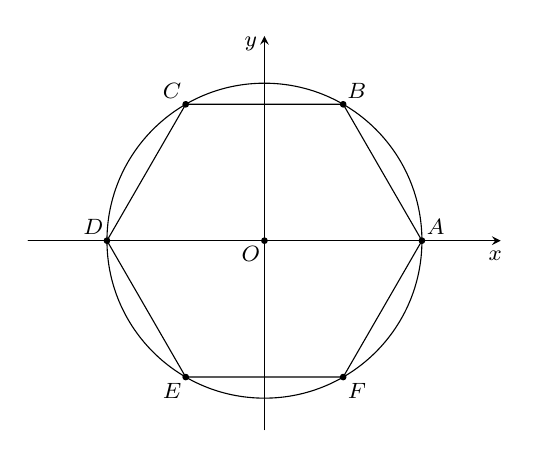
\begin{tikzpicture}[scale=2,font=\footnotesize, line join=round, line cap=round, >=stealth]
			\def \xmin{-1.5}
			\def \xmax{1.5}
			\def \ymin{-1.2}
			\def \ymax{1.3}
			\draw[->] (\xmin,0)--(\xmax,0) node[shift=(-110:0.2)] {$x$};
			\draw[->] (0,\ymin)--(0,\ymax) node[shift=(-150:0.2)] {$y$};
			\clip (\xmin,\ymin) rectangle (\xmax,\ymax);
			\path (0, 0) coordinate (O)
			(0:1) coordinate (A)
			(60:1) coordinate (B)
			(120:1) coordinate (C)
			(180:1) coordinate (D)
			(240:1) coordinate (E)
			(300:1) coordinate (F);
			\draw (A)--(B)--(C)--(D)--(E)--(F)--cycle;
			\draw (0,0) circle (1);
			\foreach \x/\goc in {A/45,B/45,C/135,D/135,E/-135,F/-45,O/-135}
			\draw[fill=black] (\x) node[shift={(\goc:7pt)}]{$\x$} circle (0.5pt);
		\end{tikzpicture}
		}
	\loigiai{
		Ta có $-\dfrac{19\pi}{3}=-\dfrac{\pi}{3}-3\cdot2\pi$.\\
		Do đó điểm biểu diễn góc lượng giác có số đo $-\dfrac{19\pi}{3}$ chính là điểm biểu diễn góc lượng giác có số đo $-\dfrac{\pi}{3}$.\\
		Vì $ABCDEF$ là lục giác điều nên $\triangle OAF$ đều suy ra $\widehat{AOF}=60^\circ$.
		Do đó điểm biểu diễn cần tìm là điểm $F$.
		}
\end{ex}
%%% TN 5
\begin{ex}[\textit{Trích đề thi GKI - trường THPT Phạm Phú Thứ - Năm học 2024-2025}]%[1D1N2-1]
	Cho $M\left(-\dfrac{1}{2};\dfrac{\sqrt3}{2}\right)$ là điểm trên đường tròn lượng giác, biểu diễn góc lượng giác có số đo $\alpha$. Khi đó, giá trị của $\sin \alpha$ bằng
	\choice
		{$-\dfrac{1}{2}$}
		{\True $\dfrac{\sqrt3}{2}$}
		{$-\dfrac{1}{\sqrt3}$}
		{$-\sqrt3$}
	\loigiai{
		Điểm $M\left(-\dfrac{1}{2}; \dfrac{\sqrt3}{2}\right)$ biểu diễn góc lượng giác có số đo $\alpha$, nên $\sin \alpha =y_0= \dfrac{\sqrt3}{2}$.
		}
\end{ex}
%%% TN 6
\begin{ex}[\textit{Trích đề thi GKI - trường THPT Chuyên Lê Quý Đôn - Năm học 2024-2025}]%[1D1N1-2]
	Đổi số đo của góc $\alpha=30^\circ$ sang rađian.
	\choice
		{$\alpha=\dfrac{\pi}{2}$}
		{$\alpha=\dfrac{\pi}{4}$}
		{\True $\alpha=\dfrac{\pi}{6}$}
		{$\alpha=\dfrac{\pi}{3}$}
	\loigiai{
		Ta có $1^\circ=\dfrac{\pi}{180}$ rad. Suy ra $30^\circ=30\cdot \dfrac{\pi}{180}=\dfrac{\pi}{6}$ rad.
		}
\end{ex}
%%% TN 7
\begin{ex}[\textit{Trích đề thi HKI  - trường THPT Chuyên Lê Quý Đôn - Năm học 2024-2025}]%[1D1N1-2]
	Một góc lượng giác có số đo là $\dfrac{\pi}{12}$ thì số đo theo đơn vị độ là bao nhiêu?
	\choice
		{$30^\circ$}
		{$10^\circ$}
		{$25^\circ$}
		{\True $15^\circ$}
	\loigiai
		{
		Ta có $\dfrac{\pi}{12}\cdot\dfrac{180}{\pi}=15^\circ$.
		}
\end{ex}
%%% TN 8
\begin{ex}[\textit{Trích đề thi GKI - trường THPT Nguyễn An Ninh - Năm học 2024-2025}]%[1D1N2-2]
	Cho biết $\dfrac{\pi}{2}<\alpha<\pi$. Khẳng định nào sau đây \textbf{sai}?
	\choice
		{$\cot\alpha<0$}
		{\True $\cos\alpha>0$}
		{$\sin\alpha>0$}
		{$\tan\alpha<0$}
	\loigiai{
		Do $\dfrac{\pi}{2}<\alpha<\pi$ suy ra  $\alpha$ thuộc góc phần tư thứ hai, nên $\sin\alpha>0$, $\cos\alpha<0$, $\tan\alpha<0$, $\cot\alpha<0$.
		}
\end{ex}
%%% TN 9
\begin{ex}[\textit{Trích đề thi HKI - trường THPT Mạc Đỉnh Chi - Năm học 2024-2025}]%[1D1N2-2]
	Cho góc $ x$ thoả $0^\circ < x <90^\circ$. Trong các mệnh đề sau, mệnh đề nào \textbf{sai}?
	\choice
		{\True $\cos x < 0$}
		{$\sin x > 0$}
		{$\tan x > 0$}
		{$\cot x > 0$}
	\loigiai{
		Do $0^\circ < x <90^\circ$ nên $ \cos x>0 $ dẫn đến $ \cos x<0 $ là mệnh đề sai.
		}
\end{ex}
%%% TN 10
\begin{ex}[\textit{Trích đề thi HKI - trường THPT Nguyễn Thị Minh Khai - Năm học 2024-2025}]%[1D1N2-1]
	Cho góc $-\dfrac{\pi}{2}< \alpha <0$, khẳng định nào sau đây đúng?
	\choice
		{\True $\sin \alpha < 0$}
		{$\cos \alpha < 0$}
		{$\tan \alpha > 0$}
		{$\cot \alpha > 0$}
	\loigiai{
		Ta có $-\dfrac{\pi}{2}< \alpha <0 \Rightarrow \sin \alpha < 0$.
		}
\end{ex}
%%% TN 11
\begin{ex}[\textit{Trích đề thi HKI - trường THPT Kẻ Sặt - Năm học 2024-2025}]%[1D1N2-2]
	Giá trị của $\tan \dfrac{\pi}{6}$ là
	\choice
		{\True $\dfrac{\sqrt3}{3}$}
		{$-\dfrac{\sqrt3}{3}$}
		{$\sqrt3$}
		{$-\sqrt3$}
	\loigiai{
		Ta có $\tan \dfrac{\pi}{6}=\dfrac{\sqrt3}{3}$.
		}
\end{ex}
%%% TN 12
\begin{ex}[\textit{Trích đề thi HKI - trường THPT Phan Bội Châu - Năm học 2024-2025}]%[1D1V2-3]
	Giá trị biểu thức $A=4\cos 2x+\sqrt2\sin 3x$, với $x=\dfrac{\pi}{4}$ là
	\choice
		{$0$}
		{$3$}
		{$\dfrac{3\sqrt2}{2}$}
		{\True $1$}
	\loigiai{
		$A=4\cos \left(2\cdot \dfrac{\pi}{4}\right)+\sqrt2\sin \left(3\cdot \dfrac{\pi}{4}\right)=4\cos \dfrac{\pi}{2} + \sqrt2\sin \dfrac{3\pi}{4}=4\cdot 0+ \sqrt2\cdot \dfrac{\sqrt2}{2}=1$.
		}
\end{ex}
%%% TN 13
\begin{ex}[\textit{Trích đề thi GKI - trường THPT Võ Thị Sáu - Năm học 2024-2025}]%[1D1H2-2]
	Cho biết $\tan\alpha=\dfrac{1}{2}$. Tính $\cot\alpha$.
	\choice
		{$\cot\alpha=-\dfrac{1}{2}$}
		{$\cot\alpha=\sqrt2$}
		{$\cot\alpha=\dfrac{1}{4}$}
		{\True $\cot\alpha=2$}
	\loigiai{Ta có $\cot\alpha=\dfrac{1}{\tan\alpha}=\dfrac{1}{\dfrac{1}{2}}=2$.
		}
\end{ex}
%%% TN 14
\begin{ex}[\textit{Trích đề thi GKI - trường THPT Tây Thạnh - Năm học 2024-2025}]%[1D1H2-2]
	Cho góc $\alpha$ thoả mãn $\cos\alpha =-\dfrac{1}{3}$ và $\dfrac{\pi}{2}<\alpha<\pi$. Tính $\sin\alpha$.
	\choice
		{$\sin\alpha=-\dfrac{2\sqrt2}{3}$}
		{\True $\sin\alpha=\dfrac{2\sqrt2}{3}$}
		{$\sin\alpha=-\dfrac{\sqrt{6}}{3}$}
		{$\sin\alpha=\dfrac{\sqrt{6}}{3}$}
	\loigiai{
		Ta có $\sin^2\alpha=1-\cos^2\alpha=1-\dfrac{1}{9}=\dfrac{8}{9}$.\\
		Do $\dfrac{\pi}{2}<\alpha <\pi$ nên $\sin\alpha =\dfrac{2\sqrt2}{3}$.
		}
\end{ex}
%%% TN 15
\begin{ex}[\textit{Trích đề thi GKI - trường THPT Nguyễn An Ninh - Năm học 2024-2025}]%[1D1H2-2]
	Cho biết $\sin\alpha = \dfrac{3}{5}$ và $-\pi<\alpha<-\dfrac{\pi}{2}$. Khẳng định nào sau đây đúng?
	\choice
		{$\cos\alpha = \dfrac{4}{5}$}
		{$\cos\alpha = \dfrac{\sqrt{34}}{5}$}
		{\True $\cos\alpha = -\dfrac{4}{5}$}
		{$\cos\alpha = -\dfrac{\sqrt{34}}{5}$}
	\loigiai{
		Ta có $\sin^2 \alpha + \cos^2 \alpha =1$ suy ra $\cos^2\alpha = 1 -\sin^2\alpha = 1-\left(\dfrac{3}{5}\right)^2 = \dfrac{16}{25}$.\\
		Do $-\pi<\alpha<-\dfrac{\pi}{2}$ nên $\alpha$ thuộc góc phần tư thứ ba, suy ra $\cos\alpha<0$.\\
		Vậy $\cos\alpha = -\dfrac{4}{5}$.
		}
\end{ex}
%%% TN 16
\begin{ex}[\textit{Trích đề thi GKI - trường THPT Trần Phú - Năm học 2024-2025}]%[1D1H2-2]
	Cho $\cos a=-\dfrac{3}{5}$ với $\pi<a<\dfrac{3\pi}{2}$, giá trị của $\cot a$ bằng
	\choice
		{$\cot a=-\dfrac{3}{4}$}
		{\True $\cot a=\dfrac{3}{4}$}
		{$\cot a=\dfrac{4}{3}$}
		{$\cot a=-\dfrac{4}{3}$}
	\loigiai{
		Ta có $\pi<a<\dfrac{3\pi}{2}$ suy ra $\sin a<0$.\\
		Khi đó $\sin^2 a+\cos^2 a=1 \Leftrightarrow \sin^2 a=1-\cos^2 a=1-\left(-\dfrac{3}{5}\right)^2=1-\dfrac{9}{25}=\dfrac{16}{25}$.\\
		Suy ra $\sin a=-\sqrt{\dfrac{16}{25}}=-\dfrac{4}{5}$.\\
		Mặt khác $\cot a=\dfrac{\cos a}{\sin a}=\dfrac{-\dfrac{3}{5}}{-\dfrac{4}{5}}=\dfrac{3}{4}$.\\
		Vậy $\cot a=\dfrac{3}{4}$.
		}
\end{ex}
%%% TN 17
\begin{ex}[\textit{Trích đề thi HKI - trường THPT Tân Châu - Năm học 2024-2025}]%[1D1N2-2]
	Cho $\tan \alpha=\sqrt{5}$, với $\pi < \alpha < \dfrac{3\pi}{2}$. Khi đó $\cos \alpha$ bằng
	\choice
		{\True $-\dfrac{\sqrt{6}}{6}$}
		{$\dfrac{1}{6}$}
		{$\sqrt{6}$}
		{$\dfrac{\sqrt{6}}{6}$}
	\loigiai{
		Ta có $\pi < \alpha < \dfrac{3\pi}{2}$, suy ra $\alpha$ thuộc góc phần tư thứ III.\\
		Trong góc phần tư thứ III, $\cos \alpha < 0$.\\
		Áp dụng công thức \allowdisplaybreaks
		\begin{eqnarray*}
			&	&1+\tan^2 \alpha=\dfrac{1}{\cos^2 \alpha}.\\
			&\Leftrightarrow	& \dfrac{1}{\cos^2 \alpha}=1+(\sqrt{5})^2=1+5=6.\\
			&\Leftrightarrow	& \cos^2 \alpha=\dfrac{1}{6}.\\
			&\Leftrightarrow	& \cos \alpha =-\dfrac{\sqrt{6}}{6}.
		\end{eqnarray*}
		}
\end{ex}
%%% TN 18
\begin{ex}[\textit{Trích đề thi HKI - trường THPT Chuyên Trần Phú - Năm học 2024-2025}]%[1D1N2-4]%
	Biết $A$, $B$, $C$ là các góc của tam giác $ABC$, khi đó
	\choice
		{$\sin C=-\sin (A+B)$}
		{$\cos C=\cos (A+B)$}
		{$\tan C=\tan (A+B)$}
		{\True $\cot C=-\cot (A+B)$}
	\loigiai{
		Xét $\triangle ABC$ ta có $\widehat{A}+\widehat{B}+\widehat{C}=\pi$, suy ra $\widehat{C}=\pi-\left(\widehat{A}+\widehat{B}\right)$. Khi đó
		$$\cot C =\cot\left(\pi-(\widehat{A}+\widehat{B})\right)=-\cot(A+B).$$
		}
\end{ex}
%%% TN 19
\begin{ex}[\textit{Trích đề thi HKI - trường THPT Hoàng Việt - Năm học 2024-2025}]%[1D1N2-4]
	Biết $\sin{a}=-\dfrac{1}{2}$, giá trị của $\sin{(\pi-a)}$ là
	\choice
		{$\sin{(\pi-a)}=\dfrac{1}{2}$}{$\sin{(\pi-a)}=-\dfrac{\sqrt3}{2}$}{\True $\sin{(\pi-a)}=-\dfrac{1}{2}$}{$\sin{(\pi-a)}=\dfrac{\sqrt3}{2}$}
	\loigiai{
		Ta có $\sin{(\pi-a)}=\sin{a}=-\dfrac{1}{2}$.
		}
\end{ex}
%%% TN 20
\begin{ex}[\textit{Trích đề thi GKII - trường THPT Tây Thạnh - Năm học 2024-2025}]%[1D1H2-4]
	Thu gọn biểu thức $A=\cos\left(\dfrac{\pi}{2}-x\right)+3\sin (\pi-x)$ ta được $A=k\sin x$. Giá trị của $k$ bằng
	\choice
		{$1$}
		{$2$}
		{$3$}
		{\True $4$}
	\loigiai{
		Ta có $A=\cos\left(\dfrac{\pi}{2}-x\right)+3\sin (\pi-x)=\sin x+3\sin x=4\sin x$.\\
		Vậy $k=4$.
		}
\end{ex}
\Closesolutionfile{ans}

\ind{PHẦN II.} \inden{Câu trắc nghiệm đúng sai. Trong mỗi ý a), b), c), d) ở mỗi câu, học sinh chọn đúng hoặc sai.}\\
\setcounter{ex}{0}
\Opensolutionfile{ans}[ans/1D1-Bai1-2-DS]
%%% ĐS 1
\begin{ex}%[1D1N2-2]
	Trên đường tròn lượng giác, cho góc lượng giác $\alpha$ có số đo $-\dfrac{1\ 041\pi}{8}$.
	\choiceTF
		{$\alpha$ thuộc góc phần tư thứ III}
		{\True $\cos\alpha>0$}
		{$\sin\alpha>0$}
		{\True $4\cot\alpha<0$}
	\loigiai{
		\begin{itemchoice}
			\itemch Ta có $-\dfrac{1\ 041\pi}{8}=-\dfrac{\pi}{8}-65\cdot2\pi$.\\
			Do góc lượng giác có số đo $-\dfrac{\pi}{8}$ thuộc góc phần tư thứ IV nên $\alpha$ cũng thuộc góc phần tư thứ IV.
			\itemch Do $\alpha$ thuộc góc phần tư thứ IV nên $\cos\alpha>0$.
			\itemch Do $\alpha$ thuộc góc phần tư thứ IV nên $\sin\alpha<0$.
			\itemch Do $\alpha$ thuộc góc phần tư thứ IV nên $\cot\alpha<0$, suy ra $4\cot\alpha<0$.
		\end{itemchoice}
		}
\end{ex}
%%% ĐS 2
\begin{ex}[\textit{Trích đề thi GKI - Trường THPT Võ Thị Sáu - Năm học 2024-2025}]%[1D1N2-2]
	Cho $\cos x=-\dfrac{3}{5}$, với $\dfrac{\pi}{2}<x<\pi$.
	\choiceTF
		{\True $\sin x>0$}
		{$\sin x=-\dfrac{4}{5}$}
		{$\cot x=-\dfrac{4}{3}$}
		{$\tan x=-\dfrac{3}{4}$}
	\loigiai{
		\begin{itemchoice}
			\itemch Do $\dfrac{\pi}{2}<x<\pi$ nên $\sin x>0$.
			\itemch Ta có $\sin^2 x=1-\cos^2 x=1-\left(-\dfrac{3}{5}\right)^2=\dfrac{16}{25}$.\\
			Do $\dfrac{\pi}{2}<x<\pi$ nên $\sin x=\dfrac{4}{5}$.
			\itemch Ta có $\cot x=\dfrac{\cos x}{\sin x}=-\dfrac{3}{4}$.
			\itemch Ta có $\tan x=\dfrac{\sin x}{\cos x}=-\dfrac{4}{3}$.
		\end{itemchoice}
		}
\end{ex}
%%% ĐS 3
\begin{ex}%[1D1H2-2]
	Trên đường tròn lượng giác, cho góc lượng giác $\alpha$ được biểu diễn tại điểm $M$ như hình.
	\begin{center}
		\begin{tikzpicture}[font=\footnotesize, >=stealth, declare function={r=1.5;}]
			\pgfmathsetmacro\goca{asin(3/5)-180}
			\path (0,0) coordinate (O) (0:r) coordinate (A) (180:r) coordinate (A') (90:r) coordinate (B) (-90:r) coordinate (B') (\goca:r) coordinate (M);
			\draw[->] (-r-0.25,0)--(r+0.5,0)node[above]{$x$};
			\draw[->] (0,-r-0.25)--(0,r+0.5)node[left]{$y$};
			\draw[->] (0:r/4) arc (0:\goca:r/4)node[right, midway]{$\alpha$};
			\fill (r,0) circle (1pt)+(-45:0.25)node{$1$};
			\draw (O) circle (r) (O)--(M);
			\foreach \x/\g in {O/135, A/45, M/\goca}{
			\fill (\x) circle (1pt)+(\g:0.25)node{$\x$};
			}
			\path
			($(O)!(M)!(A)$) coordinate (Mx) ($(O)!(M)!(B)$) coordinate (My);
			\fill (My) circle(1pt)node[right]{$-\dfrac{3}{5}$};
			\draw[dashed] (M)--(My);
		\end{tikzpicture}
	\end{center}
	\choiceTF
		{\True $\sin\alpha=-\dfrac{3}{5}$}
		{$\cos\alpha=\dfrac{4}{5}$}
		{$\tan\alpha=-\dfrac{3}{4}$}
		{$\cot\alpha=-\dfrac{4}{3}$}
	\loigiai{
		\begin{itemchoice}
			\itemch Ta có tung độ của điểm $M$ là $-\dfrac{3}{5}$ nên $\sin\alpha=-\dfrac{3}{5}$.
			\itemch Ta có $\cos^2\alpha=1-\sin^2\alpha=\dfrac{16}{25}$.\\
			Do $\alpha$ thuộc góc phần tư thứ III nên $\cos\alpha=-\dfrac{4}{5}$.
			\itemch Ta có $\tan\alpha=\dfrac{\sin\alpha}{\cos\alpha}=\dfrac{3}{4}$.
			\itemch Ta có $\cot\alpha=\dfrac{\cos\alpha}{\sin\alpha}=\dfrac{4}{3}$.
		\end{itemchoice}
		}
\end{ex}
%%% ĐS 4
\begin{ex}[\textit{Trích SGK Kết nối tri thức}]%[1D1V1-6]
	Một máy kéo nông nghiệp với bánh xe sau có đường kính là $184$ cm, bánh xe trước có đường kính là $92$ cm, xe chuyển động với vận tốc không đổi trên một đoạn đường thẳng. Biết rằng vận tốc của bánh xe sau trong chuyển động này là $80$ vòng/phút.
	\choiceTF
		{Bánh xe sau đi mỗi vòng được quãng đường có độ dài là $368\pi$ cm}
		{\True Quãng đường đi được của máy kéo trong $10$ phút là $1{,}472\pi$ km}
		{\True Vận tốc của máy kéo là $27{,}75$ km/giờ (kết quả làm tròn đến hàng phần trăm)}
		{\True Vận tốc bánh xe trước là $160$ vòng/phút}
	\loigiai{
		\begin{itemchoice}
			\itemch Bánh xe sau đi mỗi vòng được quãng đường có độ dài là $184\cdot\pi=184\pi$ (cm).
			\itemch Trong $10$ phút, bánh xe sau chuyển động được $80\cdot10=800$ vòng.\\
			Suy ra quãng đường đi được của máy kéo trong $10$ phút là $s=184\pi\cdot800=147\ 200\pi$ (cm).\\
			Hay $s=1{,}472\pi$ (km).
			\itemch Ta có $10$ phút $=\dfrac{1}{6}$ giờ.\\
			Vận tốc của máy kéo là $v=\dfrac{s}{\dfrac{1}{6}}=27{,}75$ (km/h).
			\itemch Bánh xe trước đi mỗi vòng được quãng đường $s'=92\cdot\pi=92\pi$ (cm).\\
			Số vòng bánh xe trước lăn được trong $10$ phút là $\dfrac{147\ 200\pi}{92\pi}=1\ 600$ (vòng).\\
			Suy ra vận tốc của bánh xe trước là $\dfrac{1\ 600}{10}=160$ (vòng/phút).
		\end{itemchoice}
		}
\end{ex}
%%% ĐS 5
\begin{ex}[\textit{Trích Ôn tập cuối HKI - trường THPT Nguyễn Gia Thiều - Năm học 2024-2025}]%[1D1V2-4]
	Cho biểu thức $H=\dfrac{\sin(x-2024\pi)+\cos\left(\dfrac{\pi}{2}-x\right)}{\sin(\pi-x)+\sin(\pi+x)-2}$.
	\choiceTF
		{\True $\sin(\pi-x)=\sin x$}
		{\True $\cos\left(\dfrac{\pi}{2}-x\right)=\sin x$}
		{$\sin (x-2024\pi)=-\sin x$}
		{Rút gọn biểu thức $H=0$}
	\loigiai{
		\begin{itemchoice}
			\itemch Ta có $\sin(\pi-x)=\sin x$.
			\itemch Ta có $\cos\left(\dfrac{\pi}{2}-x\right)=\sin x$.
			\itemch Ta có $\sin(x-2\ 024\pi)=\sin x$.
			\itemch $H=\dfrac{\sin (x-2\ 024\pi)+\cos \left(\dfrac{\pi}{2}-x\right)}{\sin (\pi-x)+\sin (\pi+x)-2}=\dfrac{\sin x+\sin x}{\sin x-\sin x-2}=-\sin x$.
		\end{itemchoice}
		}
\end{ex}
\Closesolutionfile{ans}

\ind{PHẦN III.} \inden{Câu trắc nghiệm trả lời ngắn. Mỗi câu học sinh ghi đáp án vào vào ô.}\\
\setcounter{ex}{0}
\Opensolutionfile{ans}[ans/1D1-Bai1-2-TLN]
%%% SA 1
\begin{ex}[\textit{Trích đề thi HKI - trường THPT Nguyễn Khuyến - Năm học 2024-2025}]%[1D1N1-4]
	Cho đường tròn bán kính $r = 5$. Tính độ dài của cung tròn có số đo $\dfrac{\pi}{8}$. (kết quả làm tròn đến hàng phần trăm)
	\par\shortans{$1{,}96$}
\loigiai{
	Độ dài cung tròn có số đo $\dfrac{\pi}{8}$ là $\ell= 5\cdot \dfrac{\pi}{8} = \dfrac{5\pi}{8} \approx 1{,}96$.
	}
\end{ex}
%%% SA 2
\begin{ex}[\textit{Trích đề thi HKI - trường THPT Tân Châu - Năm học 2024-2025}]%[1D1N2-2]
	Cho góc lượng giác $\alpha=210^\circ$, trong số các giá trị lượng giác $\sin \alpha$, $\cos \alpha$, $\tan \alpha$, $\cot \alpha$ có bao nhiêu giá trị là số dương?
	\par\shortans{$2$}
\loigiai{
	Góc lượng giác $\alpha=210^\circ$ nằm ở góc phần tư thứ III. Nên $\sin \alpha<0$, $\cos \alpha<0$, $\tan \alpha>0$, $\cot \alpha>0$.\\
	Vậy có $2$ giá trị là số dương.
	}
\end{ex}
%%% 5 câu

%%% SA 3
\begin{ex}[\textit{Trích đề thi GKI - trường THPT Chuyên Bình Thuận - Năm học 2024-2025}]%[1D1H1-6]
	Một vòng quay Mặt Trời trong trò chơi cảm giác mạnh tại một khu du lịch, quay mỗi vòng mất $15$ phút. Tại vị trí quan sát, bạn Hoa thấy vòng quay chuyển động theo chiều kim đồng hồ. Khi vòng quay chuyển động được $10$ phút, bán kính của vòng quay quét một góc lượng giác có số đo bằng $-\dfrac{a\pi}{b}$ (rad) (trong đó $\dfrac{a}{b}$ là phân số tối giản và $a$, $b > 0$). Tính $a + b$.
	\par\shortans{$7$}
\loigiai{
	Do vòng quay Mặt Trời quay mỗi vòng khoảng $15$ phút và chuyển động theo chiều kim đồng hồ nên sau $15$ phút, bán kính của vòng quay quét một góc lượng giác có số đo bằng $-2\pi$ (rad).\\
	Do đó, sau $10$ phút, bán kính của vòng quay quét một góc lượng giác có số đo bằng
	$$\dfrac{-2\pi}{15}\cdot 10 = -\dfrac{4\pi}{3} \textrm{ (rad).}$$
	Vậy $a = 4$ và $b = 3$, suy ra $a + b = 4 + 3 = 7$.
	}
\end{ex}
%%% SA 4
\begin{ex}[\textit{Trích đề thi GKI - trường THPT Nguyễn An Ninh - Năm học 2024-2025}]%[1D1V2-5]
	Một xe đạp đang di chuyển, van $M$ của bánh xe quay quanh trục $O$ theo chiều kim đồng hồ với tốc độ góc không đổi $10$ rad/s. Khoảng cách từ van $M$ đến mặt đất là đoạn $MH$. Ban đầu, van $M$ nằm ở vị trí $A$ (xem hình). Hỏi sau 2 phút khoảng cách từ van $M$ đến mặt đất là bao nhiêu cm? Biết bán kính bánh xe $R = 35$ cm. Giả sử độ dày của lốp xe không đáng kể. Làm tròn kết quả đến hàng phần mười.
	\begin{center}
		\begin{tikzpicture}
			% Vẽ mặt đất
			\draw[thick] (-4,-2) -- (4,-2) node[anchor=north] {Mặt đất};
			% Vẽ trục x và trục y
			\draw[->] (-3,0) -- (3,0) node[anchor=north west] {$x$};
			\draw[->] (0,-2) -- (0,3) node[anchor=east] {$y$};
			% Vẽ bánh xe
			\draw[thick] (0,0) circle (2);
			% Vẽ bán kính OM và đoạn thẳng AH
			\draw[thick] (1.3,1.5) -- (1.3,-2) node[below] {H};
			\draw[thick] (0,0) -- (2,0) node[anchor=north west] {A};
			\draw[thick] (0,0) -- (1.3,1.5) node[above right] {M};
			% Đặt các điểm O và các kí hiệu
			\node at (0,0) [below left] {O};
			\node at (0.4,0.182) {$\alpha$};
		\end{tikzpicture}
	\end{center}
	\par\shortans{$2$}
\loigiai{
	Góc quay sau $2$ phút là $\theta = \omega \cdot t = 10 \cdot 120 = 1\ 200$ (rad).\\
	Số vòng quay $M$ sau $2$ phút là $\dfrac{1\ 200}{2\pi} \approx 191$ (vòng).\\
	Sau mỗi vòng quay, van $M$ sẽ trở lại vị trí ban đầu, vì vậy sau $191$ vòng quay, van $M$ trở lại vị trí ban đầu.\\
	Khi $M$ ở vị trí $A$, khoảng cách từ van $M$ đến mặt đất là $MH = R = 35$ (cm).
	}
\end{ex}
%%% SA 5
\begin{ex}[\textit{Trích đề thi GHI - trường THPT Nguyễn Thái Bình - Năm học 2024-2025}]%[1D1C1-6]
	Trong hình dưới đây, vi trí cabin mà Bình và Cường ngồi trên đu quay được đánh dấu lần lượt tại điểm $B$ và $C$. Tâm $O$ cách măt đất một khoảng $h=13 \mathrm{~m}$, số đo của một góc lượng giác có tia đầu $O A$, tia cuối $O B$ là $\alpha=-30^\circ, O C \perp O B$, độ cao của điểm $C$ so với mặt đất là $7 \mathrm{~m}$. Tính bán kính $R$ của đu quay (biết vi trí $C$ gần mặt đất hơn so với vị trí của $B$). Kết quả làm tròn đến một chữ số thập phân.
	\begin{center}
		\begin{tikzpicture}[scale=0.7,>=stealth]
			\def\r{3}
			\def\a{\r/10}
			\def\n{12}%Số nan đu quay
			\def\m{12}%Số lồng đu quay
			\pgfmathsetmacro{\g}{20}
			\pgfmathsetmacro{\b}{2*\a/3}
			\pgfmathsetmacro{\xo}{\a *cos(\g)}
			\pgfmathsetmacro{\yo}{\b *sin(\g)}
			\def\longdq(#1:#2){
			\begin{scope}[shift={(#1:#2)}]
				\draw (0,-\b) ellipse ({\b/2} and {\b});
				\fill[blue!60] (\xo,\yo-\b) arc (\g:-180-\g:{\a} and {\b})--cycle;
				\draw (0,-\b) ellipse({\a} and {\b});
			\end{scope}
			}
			\foreach \i in {1,...,\n}{
			\pgfmathsetmacro{\gm}{360*\i/\n}
			\pgfmathsetmacro{\gh}{(360*\i+180)/\n}
			\pgfmathsetmacro{\gb}{360*(\i+1)/\n}
			\draw (\gm:\r-\a)--(\gh:\r)--(\gb:\r-\a);
			\draw (\gm:\r-\a)--(\gm:\a);
			}
			\draw[double] (0:0) circle (\r);
			\draw (0:0) circle (\r-\a);
			\foreach \i in {1,...,\m}{\longdq(360*\i/\m:\r)}
			\draw[top color =gray!10, bottom color=gray!30] (-30:\a) arc(-30:0:\a) --(-70:1.5*\r)--++(\a/2,0)--([turn]-70:\r/2) --([turn]-110:3*\a)--(-30:\a);
			\draw[top color =gray!10, bottom color=gray!30, xscale=-1] (-30:\a) arc(-30:0:\a) --(-70:1.5*\r)--++(\a/2,0)--([turn]-70:\r/2) --([turn]-110:3*\a)--(-30:\a);
			\fill[ball color=orange] (0:0) circle (\a);
			\draw[double] (0:0) circle (\a);
			\draw[->] (-4,0)--(6.5,0) node[below]{$x$};
			\draw[->] (0,-6)--(0,4) node[right]{$y$};
			\draw (0,0) node[above left]{$O$};
			\coordinate (O) at (0,0);
			\coordinate (A) at ($(O) + (0:3)$);
			\coordinate (B) at ($(O) + (-30:3)$);
			\coordinate (C) at ($(O) + (240:3)$);
			\coordinate (P) at ($(O) + (270:3)$);
			\path
			($(O)!(C)!(P)$)coordinate (K);
			\draw[line width=1.3pt,red] (A)--(O)--(B) (O)--(C);
			\foreach \x/\g in {A/50,B/0,C/180}\draw[fill=black] (\x) circle (.05) +(\g:.5)node{\footnotesize$\x$};
			\draw [shift={(0,0)},->,line width=0.3pt] (0:.9) arc (0:-30:.9) node[right]{\scriptsize$\alpha$};
			\draw[dashed] (0,3)--(5,3);
			\draw[dashed] (0,-5.66)--(5,-5.66)node[below]{\text{ Mặt đất}};
			\draw[<->] (4,0)--(4,-5.66)node[pos=.5,right]{\footnotesize$h=13$ m};
			\draw[<->] (4,0)--(4,3)node[pos=.5,right]{\footnotesize$R$ m};
			\draw pic[draw,red,line width=1.3pt,angle radius=2mm] {right angle = B--O--C};
		\end{tikzpicture}
	\end{center}
	\par\shortans{$6{,}9$}
\loigiai{
	\begin{center}
		\begin{tikzpicture}[scale=0.7,>=stealth]
			\def\r{3}
			\def\a{\r/10}
			\def\n{12}%Số nan đu quay
			\def\m{12}%Số lồng đu quay
			\pgfmathsetmacro{\g}{20}
			\pgfmathsetmacro{\b}{2*\a/3}
			\pgfmathsetmacro{\xo}{\a *cos(\g)}
			\pgfmathsetmacro{\yo}{\b *sin(\g)}
			\def\longdq(#1:#2){
			\begin{scope}[shift={(#1:#2)}]
				\draw (0,-\b) ellipse ({\b/2} and {\b});
				\fill[blue!60] (\xo,\yo-\b) arc (\g:-180-\g:{\a} and {\b})--cycle;
				\draw (0,-\b) ellipse({\a} and {\b});
			\end{scope}
			}
			\foreach \i in {1,...,\n}{
			\pgfmathsetmacro{\gm}{360*\i/\n}
			\pgfmathsetmacro{\gh}{(360*\i+180)/\n}
			\pgfmathsetmacro{\gb}{360*(\i+1)/\n}
			\draw (\gm:\r-\a)--(\gh:\r)--(\gb:\r-\a);
			\draw (\gm:\r-\a)--(\gm:\a);
			}
			\draw[double] (0:0) circle (\r);
			\draw (0:0) circle (\r-\a);
			\foreach \i in {1,...,\m}{\longdq(360*\i/\m:\r)}
			\draw[top color =gray!10, bottom color=gray!30] (-30:\a) arc(-30:0:\a) --(-70:1.5*\r)--++(\a/2,0)--([turn]-70:\r/2) --([turn]-110:3*\a)--(-30:\a);
			\draw[top color =gray!10, bottom color=gray!30, xscale=-1] (-30:\a) arc(-30:0:\a) --(-70:1.5*\r)--++(\a/2,0)--([turn]-70:\r/2) --([turn]-110:3*\a)--(-30:\a);
			\fill[ball color=orange] (0:0) circle (\a);
			\draw[double] (0:0) circle (\a);
			\draw[->] (-4,0)--(6.5,0) node[below]{$x$};
			\draw[->] (0,-6)--(0,4) node[right]{$y$};
			\draw (0,0) node[above left]{$O$};
			\coordinate (O) at (0,0);
			\coordinate (A) at ($(O) + (0:3)$);
			\coordinate (B) at ($(O) + (-30:3)$);
			\coordinate (C) at ($(O) + (240:3)$);
			\coordinate (P) at ($(O) + (270:3)$);
			\path
			($(O)!(C)!(P)$)coordinate (K);
			\draw[line width=1.3pt,red] (A)--(O)--(B) (O)--(C);
			\draw[dashed,line width=1pt] (C)--(K);
			\foreach \x/\g in {A/50,B/0,C/180,K/20}\draw[fill=black] (\x) circle (.05) +(\g:.4)node{\footnotesize$\x$};
			\draw [shift={(0,0)},->,line width=0.3pt] (0:.9) arc (0:-30:.9) node[right]{\scriptsize$\alpha$};
			\draw[dashed] (0,3)--(5,3);
			\draw[dashed] (0,-5.66)--(5,-5.66)node[below]{\text{ Mặt đất}};
			\draw[<->] (4,0)--(4,-5.66)node[pos=.5,right]{\footnotesize$h=13$ m};
			\draw[<->] (4,0)--(4,3)node[pos=.5,right]{\footnotesize$R$ m};
			\draw pic[draw,red,line width=1.3pt,angle radius=2mm] {right angle = B--O--C};
			\draw pic[draw,line width=1.0pt,angle radius=2mm] {right angle = O--K--C};
			\draw (0,-5.66) node[left]{$H$};
		\end{tikzpicture}
	\end{center}
	Gọi $H$, $K$ là điểm như hình vẽ.\\
	Bạn Cường đã quay một góc $\alpha =-120^\circ$.\\
	Khi đó $C\left(R\cos \left(-120^\circ\right);R\sin\left(-120^\circ\right)\right)\Rightarrow \overline{OK}=R\sin \left(-120^\circ\right)$.\\
	Mà $OK=OH-HK=13-7=6\Rightarrow \overline{OK}=-6$.\\
	Vậy $R\sin \left(-120^\circ\right)=-6\Rightarrow R=\dfrac{-6}{\sin \left(-120^\circ\right)}=4\sqrt3\approx 6{,}9\mathrm{~m}$.\\
	Vậy $R=6{,}9\mathrm{~m}$.
	}
\end{ex}
\Closesolutionfile{ans}

\ind{PHẦN IV.} \inden{Tự luận.}\\
\setcounter{ex}{0}
\Opensolutionfile{ans}[ans/1D1-Bai1-2-TL]
%%% TL 1
\begin{ex}[\textit{Trích đề thi GKI - trường THPT Trần Khai Nguyên - Năm học 2023-2024}]%[1D1N1-5]
	Xác định điểm $M$ và $N$ trên đường tròn lượng giác lần lượt là điểm biểu diễn của các góc lượng giác có số đo bằng $-135^\circ$, $\dfrac{9\pi}{4}$.
\loigiai{
	\begin{center}
		\begin{tikzpicture}[line join = round, line cap = round, >=stealth, font=\footnotesize, scale=0.8]
			\tikzset{label style/.style={font=\footnotesize}}
			\path (0,0) coordinate (O)
			(3,0) coordinate (A)
			(0:0)++(-135:3) coordinate (M)
			(0:0)++(45:3) coordinate (N)
			;
			\draw[->] (-4,0) -- (4,0) node[above,blue]{$x$};
			\draw[->] (0,-4) -- (0.,4) node[left,blue]{$y$};
			\draw (O) circle (3cm);
			\draw[red,-stealth,smooth,samples=100] plot[domain =0:(9/4)*pi]({.6*(1.12)^(\x) *cos(\x r)},{.6*(1.12)^(\x)*sin(\x r)});
			\draw[blue,-stealth,smooth,samples=100] plot[domain =0:(-3/4)*pi]({1.5*(1.12)^(\x) *cos(\x r)},{1.5*(1.12)^(\x)*sin(\x r)});
			\draw[red] (O)--(N);
			\draw[blue] (O)--(M);
			\foreach \p/\r in {A/-45,M/-100,N/40,O/-40}
			\fill (\p) circle (1pt) node[shift={(\r:3mm)},blue]{$\p$};
			\draw (25:2)node{$\dfrac{9\pi}{4}$} (-50:2)node{$-135^\circ$};
		\end{tikzpicture}
	\end{center}
	}
\end{ex}
%%% TL 2
\begin{ex}[\textit{Trích đề thi GKI - trường THPT Nam Kỳ Khởi Nghĩa - Năm học 2023-2024}]%[1D1H2-2]
	Cho $\sin x=-\dfrac{\sqrt3}{4}$ và $x \in\left(\pi ; \dfrac{3 \pi}{2}\right)$. Tính giá trị của $\cos x$, $\tan x$.
\loigiai
	{Ta có $\sin^2x+\cos^2x=1$ nên $\cos^2x=1-\sin^2x=1-\dfrac{3}{16}=\dfrac{13}{16}\Rightarrow \cos x=\pm\dfrac{\sqrt{13}}{4}$.\\
	Do $x\in\left(\pi; \dfrac{3\pi}{2}\right)$ nên $\cos x<0$, ta chọn $\cos x=-\dfrac{\sqrt{13}}{4}$.\\
	Từ đó suy ra
	$\tan x =\dfrac{\sin x }{\cos x}=\dfrac{-\dfrac{\sqrt3}{4}}{-\dfrac{\sqrt{13}}{4}}=\dfrac{\sqrt{39}}{13}$.\\
	Vậy giá trị  $\cos x= -\dfrac{\sqrt{13}}{4}$ và $\tan x=\dfrac{\sqrt{39}}{13}$.
	}
\end{ex}
%%% TL 3
\begin{ex}[\textit{Trích đề thi HKI- trường THPT Nguyễn Huệ - Năm học 2023-2024}]%[1D1H2-2]
	Cho $\cos \alpha=-\dfrac{2}{3}$, $\dfrac{\pi}{2} < \alpha < \pi$. Tính các giá trị lượng giác còn lại của góc $\alpha$.
\loigiai{
	Do $\dfrac{\pi}{2}<\alpha<\pi$ nên $\sin \alpha>0$. Khi đó
	\allowdisplaybreaks
	\begin{eqnarray*}
		& 	&\sin \alpha=\sqrt{1-\cos ^2 \alpha}=\sqrt{1-\dfrac{4}{9}}=\dfrac{\sqrt{5}}{3} \\
		& 	&\tan \alpha=\dfrac{\sin \alpha}{\cos \alpha}=\dfrac{\sqrt{5}}{3}: \dfrac{-2}{3}=\dfrac{-\sqrt{5}}{2} \\
		& 	&\cot \alpha=\dfrac{1}{\tan \alpha}=\dfrac{-2 \sqrt{5}}{5} .
	\end{eqnarray*}
	}
\end{ex}
%%% TL 4
\begin{ex}[\textit{Trích đề thi GKI - trường THPT Bùi Thị Xuân - Năm học 2023-2024}]%[1D1H2-2]
	Cho $\tan \alpha=3$ với $0^\circ<\alpha<90^\circ$. Tính $\cot \alpha,$ $\cos \alpha,$ $\sin \alpha$.
\loigiai{
	Ta có $ \cot \alpha  =\dfrac{1}{\tan \alpha }= \dfrac{1}{3}$.\\
	Ta lại có $\dfrac{1}{\cos^2\alpha}=1+\tan^2\alpha=1+3^2=10 \Rightarrow \cos^2\alpha=\dfrac{1}{10}\Rightarrow \cos\alpha=\pm\dfrac{\sqrt{10}}{10}$.\\
	Do $0^\circ<\alpha<90^\circ$ nên $\cos \alpha>0$, do đó $\cos\alpha=\dfrac{\sqrt{10}}{10}.$\\
	Từ đó suy ra $\sin \alpha = \tan \alpha \cdot \cos \alpha = 3\cdot \dfrac{\sqrt{10}}{10} = \dfrac{3\sqrt{10}}{10}. $
	}
\end{ex}
%%% TL 5
\begin{ex}[\textit{Trích đề thi GKI - Trường THPT Năng Khiếu - Năm học 2023-2024}]%[1D1H2-2]
	\begin{enumerate}
		\item Cho $\sin x=-\dfrac{1}{3}$ và $\pi <x<\dfrac{3\pi}{2}$. Tính giá trị của $P=\dfrac{2\sin x\cos x}{3 \cos^2x+1}$.
		\item Cho $\cot x=3$. Tính giá trị của $Q=\dfrac{\cos x +2\sin x}{3\cos x-\sin x}$.
	\end{enumerate}
\loigiai{
	\begin{enumerate}
		\item Vì $ \pi <x<\dfrac{3\pi}{2} $ nên $ \cos x <0 $.
		Do đó $ \cos x=-\sqrt{1-\sin^2x}=-\sqrt{1-\left(-\dfrac{1}{3}\right)^2}=-\dfrac{2\sqrt2}{3} $.\\
		Suy ra $P=\dfrac{2\sin x\cos x}{3\cos^2x+1}=\dfrac{2\cdot\left(-\dfrac{1}{3}\right)\left(-\dfrac{2\sqrt2}{3}\right)}{3\cdot\left(-\dfrac{2\sqrt2}{3}\right)^2+1}=\dfrac{4\sqrt2}{33}$.
		\item $ Q=\dfrac{\cos x +2 \sin x}{3 \cos x-\sin x}=\dfrac{\dfrac{\cos x}{\sin x}+2}{3\cdot\dfrac{\cos x}{\sin x}-1}=\dfrac{\cot x+2}{3\cot x-1}=\dfrac{3+2}{3\cdot3-1}=\dfrac{5}{8} $.
	\end{enumerate}
	}
\end{ex}
%%% TL 6
\begin{ex}[\textit{Trích đề thi GKI - trường THPT Hiệp Hòa - Năm học 2023-2024}]%[1D1H2-2]
	Tính giá trị các biểu thức sau $A=\sin\dfrac{7\pi}{6}+\cos9\pi+\tan\left(-\dfrac{5\pi}{4}\right)+\cot\dfrac{7\pi}{2}$.
\loigiai{
	Ta có
	\begin{eqnarray*}
		A	&=	&\sin\dfrac{7\pi}{6}+\cos 9\pi+\tan\left(-\dfrac{5 \pi}{4}\right)+\cot\dfrac{7\pi}{2}\\
		&=	&\sin\left(\pi+\dfrac{\pi}{6}\right)+\cos(8\pi+\pi)-\tan\left(\pi+\dfrac{\pi}{4}\right)+\cot\left(3\pi+\dfrac{\pi}{2}\right)\\
		&=	&-\sin\dfrac{\pi}{6}+\cos\pi-\tan\dfrac{\pi}{4}+\cot\dfrac{\pi}{2}\\
		&=	&-\dfrac{1}{2}-1-1+0\\
		&=	&-\dfrac{5}{2}.
	\end{eqnarray*}
	}
\end{ex}
%%% TL 7
\begin{ex}[\textit{Trích đề thi GKI - trường THPT Thủ Đức - Năm học 2023-2024}]%[1D1H2-3]
	Rút gọn biểu thức $A=\cos^2\left(\dfrac{234^{97}\pi+x}{133}\right)+\sin^2 \left(\dfrac{234^{97}\pi+x}{133}\right)+2\tan\left(117^{98}\pi\right)$.
\loigiai{
	Ta có: $
	\begin{aligned}[t]
		A	&=\cos^2\left(\dfrac{234^{97}\pi+x}{133}\right)+\sin^2\left(\dfrac{234^{97}\pi+x}{133}\right)+2\tan\left(117^{98}\pi\right)\\
		&=1+2\tan\left(k\pi\right)\\
		&=1+2\cdot0\\
		&=1.
	\end{aligned}
	$\\
	Vậy $A=1$.
	}
\end{ex}
%%% TL 8
\begin{ex}[\textit{Trích đề thi GKI - trường THPT Ngô Quyền - Năm học 2023-2024}]%[1D1H1-6]
	Bánh xe của người đi xe đạp quay được $11$ vòng trong $8$ giây. Tính góc (theo rađian) mà bánh xe quay được trong một giây và quãng đường mà người đi xe đạp đã đi được trong $2$ phút biết rằng đường kính của xe đạp là $700$ mm.
\loigiai{
	Số đo góc mà bánh xe quay được trong $8$ giây là $11\cdot 2\pi = 22\pi$ (rađian).\\
	Số đo góc mà bánh xe quay được trong $1$ giây là $\dfrac{22\pi}{8} = \dfrac{11\pi}{4}$ (rađian).\\
	Đổi đơn vị $2$ phút $= 120$ giây.\\
	Số vòng bánh xe đạp quay được trong $2$ phút là $\dfrac{120\cdot 11}{8} = 165$ vòng.\\
	Quãng đường mà người đi xe đạp đã đi được trong $2$ phút là $165\cdot \pi\cdot 700 \approx 362\ 853{,}95$ mm.
	}
\end{ex}
%%% TL 9
\begin{ex}[\textit{Trích đề thi GKI - trường THPT Nguyễn Chí Thanh - Năm học 2023-2024}]%[1D1H1-6]
	\immini
	{Trên đồng hồ có kim chỉ giờ dài $6 $ cm có gắn một con rùa ở đầu kim và kim chỉ phút dài $11$ cm có gắn một con thỏ ở đầu kim. Tại thời điểm quan sát đồng hồ đang chỉ $4$ giờ đúng. Tính hiệu quãng đường của thỏ và rùa đi được tính từ lúc $4$ giờ đúng đến $5$ giờ đúng.}{
	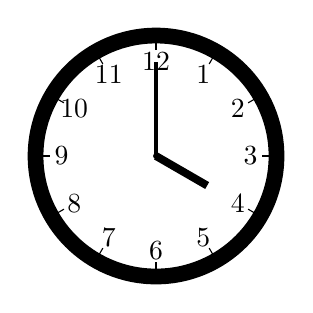
\begin{tikzpicture}[scale=0.3]
		\def\hours{0}
		\def\minutes{0}
		\def\seconds{0}
		\draw[line width=0.2cm] (0,0) circle (5.1cm);
		% Minutes
		\foreach \i in {1,2,...,60}{
		\def\angle{\i*6}
		\draw[thin] (\angle:5cm) -- (\angle:4.9cm);
		}
		% 5 minutes
		\foreach \i in {1,2,...,12}{
		\def\angle{\i*-30+90}
		\draw[thin] (\angle:5cm) -- (\angle:4.5cm);
		\node at (\angle:4cm) {\i};
		};
		% Hour hand
		\def\angle{\hours*-30 + \minutes*-0.5 + \seconds*-0.008333 -180}
		\draw[line width=0.1cm] (0,0) -- (-30:2.5cm);
		% Minute hand
		\def\angle{\minutes*-6 + \seconds*-0.1 +90}
		\draw[line width=0.05cm] (0,0) -- (\angle:4cm);
		%% Second hand
		% \def\angle{\seconds*-6+90}
		% \draw[very thick,color=red] (\angle:-1cm) -- (\angle:4.5cm);
		% \draw[line width=0.1cm,color=red] (\angle:-1cm) -- (\angle:-0.25cm);
		% Center dot
		\draw[fill=black] (0,0) circle (0.1cm);
	\end{tikzpicture}
	}
\loigiai{
	Ta có đồng hồ được chia thành $12$ phần bằng nhau nên mỗi phần là $\dfrac{360^\circ}{12}=30^\circ$.\\
	Kim giờ quay được một giờ thì quãng đường con rùa đi được là $\dfrac{\pi \cdot 6 \cdot 30^\circ}{180^\circ}=\pi$.\\
	Kim phút sau mộ giờ quay được 1 vòng nên quãng đường con thỏ đi được là $2\pi \cdot 11=22\pi$.\\
	Vậy hiệu quãng đường đi được là $22\pi - \pi =21 \pi$.
	}
\end{ex}
%%% TL 10
\begin{ex}[\textit{Trích SBT Chân trời sáng tạo}]%[1D1V1-6]
	\immini
	{Một chiếc quạt trần năm cánh quy với tốc độ $175$ vòng/phút. Chọn chiều quay của quạt là chiều dương. Xét một cánh quạt trong năm cánh.
	\begin{enumerate}
		\item Sau $5$ giây, cánh quạt đó quay được một góc có số đo bao nhiêu radian?
		\item Sau thời gian bao lâu cánh quạt đó quay được một góc có số đo $42\pi$?
	\end{enumerate}
	}
	{
	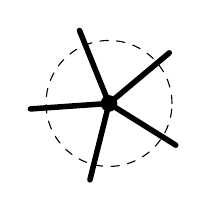
\begin{tikzpicture}[font=\footnotesize, line join=round, line cap=round, >=stealth, scale=1]
		\def\r{1}
		\path (0,0) coordinate (O);
		\draw[dashed] (O) circle (\r-0.2);
		\foreach \i in {1,...,5}{\draw[line width=2pt] (O)--(40+360*\i/5:\r);}
		\fill (O) circle (3pt);
	\end{tikzpicture}
	}
\loigiai{
	\begin{enumerate}
		\item Tốc độ $175$ vòng/phút đồng nghĩa với cánh quạt quay được $175\cdot2\pi=350\pi$ (rad) trong $60$ giây.\\
		Suy ra trong $5$ giây cánh quạt quay được một góc lượng giác có số đo $\dfrac{350\pi\cdot5}{60}=\dfrac{175\pi}{6}$.
		\item Vận tốc góc của cánh quạt là $\dfrac{350\pi}{60}=\dfrac{35\pi}{6}$ (rad/giây).\\
		Thời gian cánh quạt quay được một góc có số đo $42\pi$ là $\dfrac{42\pi}{\dfrac{35\pi}{6}}=7{,}2$ (giây).
	\end{enumerate}
	}
\end{ex}
\Closesolutionfile{ans}